%\documentclass[fontset = none, t, aspectratio=169]{ctexbeamer}
\documentclass[fontset = none, t, aspectratio=169]{ctexbeamer}

% 修改自萧山主题的凤岗主题
\usetheme{nwafufengang}

% 载入需要的宏包
% 加载宏包
%===================注意======================%
% 在调用beamer.cls宏包后,以下宏包将自动调用,
% 不应单独调用这些宏包,以免发生冲突
% amsfonts, amsmath, amssymb, amsthm, 
% enumerate, geometry, graphics, graphicx, 
% hyperref, url, 
% ifpdf, keyval, xcolor, xxcolor
% =============================================%
% % 调整行间距
\usepackage{setspace}

% 生成二维码
\usepackage{qrcode}

% 加载需要的宏包
\usepackage{csquotes}

% 符号字体
\usepackage{fontawesome5}

% unicode数学符号
\usepackage{unicode-math}

\usepackage{multicol}

% ========排版键盘组合和菜单的宏包=========
\usepackage{menukeys}

% ========图像标注宏包=========
%\usepackage{tikz-imagelabels}
\usepackage{tikz-imglabels}
% =========调整项目列表格式=========
%\usepackage{enumitem}

%tikz-imagelabels

%%% Local Variables: 
%%% mode: latex
%%% TeX-master: "../main.tex"
%%% End:


% 进行必要的设置
% 载入字体(需要安装相应字体)
\setmainfont{LibertinusSerif}[% 英文字体
  Extension      = .otf,
  UprightFont    = *-Regular,
  BoldFont       = *-Bold,
  ItalicFont     = *-Italic,
  BoldItalicFont = *-BoldItalic,
  Scale          = 1.0]
%\setmonofont{Iosevka}[Scale=1.0]% 等宽字体,主要用于代码排版
%\setmonofont{Iosevka Term}% 英文等宽字体,主要用于代码排版
\setmathfont{LibertinusMath-Regular.otf}% Iosevka数学字体,需要unicode-math支持
\setCJKmainfont{Source Han Serif SC}[ % 中文衬线字体,思源宋体
  UprightFont     = * SemiBold,
  BoldFont        = * Heavy,
  ItalicFont      = * Light,
  BoldItalicFont  = * Medium,
  RawFeature      = +fwid]
\setCJKsansfont{Source Han Sans SC}[ % 中文无衬线字体,思源宋体
  UprightFont     = * Medium,
  BoldFont        = * Heavy,
  ItalicFont      = * Light,
  BoldItalicFont  = * Normal,
  RawFeature      = +fwid]  
\setCJKmonofont{Sarasa Mono SC}[% 中文等宽字体,Sarasa Mono SC
  UprightFont     = * Medium,
  BoldFont        = * Medium,
  ItalicFont      = * Extralight,
  BoldItalicFont  = * Light,
  RawFeature      = +fwid]   

%% 自定义相关的名称宏命令
%% ==================================================
%% \newcommand{\yourcommand}[参数个数]{内容}
% 西北农林科技大学各单位名称
\newcommand{\nwafu}{西北农林科技大学}
\newcommand{\cie}{信息工程学院}
\newcommand{\ca}{农学院}
\newcommand{\cpp}{植物保护学院}
\newcommand{\ch}{园艺学院}
\newcommand{\cast}{动物科技学院}
\newcommand{\cvm}{动物医学院}
\newcommand{\cf}{林学院}
\newcommand{\claa}{风景园林艺术学院}
\newcommand{\cnre}{资源环境学院}
\newcommand{\cwrae}{水利与建筑工程学院}
\newcommand{\cmee}{机械与电子工程学院}
\newcommand{\cfse}{食品科学与工程学院}
\newcommand{\ce}{葡萄酒学院}
\newcommand{\cls}{生命科学学院}
\newcommand{\cs}{理学院}
\newcommand{\ccp}{化学与药学院}
\newcommand{\cem}{经济管理学院}
\newcommand{\cm}{马克思主义学院}
\newcommand{\dfl}{外语系}
\newcommand{\iec}{创新实验学院}
\newcommand{\ci}{国际学院}
\newcommand{\dpe}{体育部}
\newcommand{\cvae}{成人教育}
\newcommand{\iswc}{水土保持研究所}

%% 签署春秋学期日期命令
\newcommand{\tomonth}{
  \the\year 年\the\month 月
}


\newcommand{\tomonthen}{
  \ifcase\the\month
  \or January%
  \or February%
  \or March%
  \or April%
  \or May%
  \or June%
  \or July%
  \or August%
  \or September%
  \or October%
  \or November%
  \or December%
  \fi, \the\year
}

\newcommand{\tosemester}{
  \the\year 年\ 
  \ifcase\the\month
  \or 秋%
  \or 春%
  \or 春%
  \or 春%
  \or 春%
  \or 春%
  \or 春%
  \or 夏%
  \or 秋%
  \or 秋%
  \or 秋%
  \or 秋%
  \fi 
}

\newcommand{\tosemesteren}{  
  \ifcase\the\month
  \or Autumn%
  \or Spring%
  \or Spring%
  \or Spring%
  \or Spring%
  \or Spring%
  \or Summer%
  \or Autumn%
  \or Autumn%
  \or Autumn%
  \or Autumn%
  \or Autumn%
  \fi, \the\year
}

% 插图路径设置
% ==================================================
\graphicspath{{figs/}}%图片所在的目录
% ==================================================

%改变脚注的符号
\setbeamerfont{footnote}{size=\zihao{7}} % 改变脚注字号
\makeatletter
\def\@fnsymbol#1{\ensuremath{\ifcase#1\or *\or \dagger\or \ddagger\or
   \mathsection\or \mathparagraph\or \|\or **\or \dagger\dagger
   \or \ddagger\ddagger \else\@ctrerr\fi}}
\makeatother
\renewcommand{\thefootnote}{\fnsymbol{footnote}}

\DeclareRobustCommand{\nonumberfootnote}[2][]{%
  \let\thefootnote\relax
  \footnotetext#1{#2}}    

\makeatletter
\def\@fnsymbol#1{\ensuremath{\ifcase#1\or *\or \dagger\or \ddagger\or
   \mathsection\or \mathparagraph\or \|\or **\or \dagger\dagger
   \or \ddagger\ddagger \else\@ctrerr\fi}}
\renewcommand{\thefootnote}{\fnsymbol{footnote}}
\makeatother

% PoZheHao, see https://github.com/CTeX-org/ctex-kit/issues/382
\ExplSyntaxOn
\xeCJK_new_class:n { PoZheHao }
\__xeCJK_save_CJK_class:n { PoZheHao }
\xeCJK_declare_char_class:nn { PoZheHao } { "2014 }
\seq_map_inline:Nn \g__xeCJK_class_seq
  {
    \str_if_eq:nnF {#1} { PoZheHao }
      {
        \xeCJK_copy_inter_class_toks:nnnn { PoZheHao } {#1} { FullRight } {#1}
        \xeCJK_copy_inter_class_toks:nnnn {#1} { PoZheHao } {#1} { FullRight }
      }
  }
\ExplSyntaxOff

% 超链接及符号
\newcommand\link[1]{\href{#1}{\ \faExternalLinkSquare*}}  

% TikZ宏包扩展
\usetikzlibrary{fit}
% \usetikzlibrary{graphs}
% \usetikzlibrary{mindmap,trees}
%Here we change the style for all concepts: (Stefan K.)
% \tikzset{every concept/.style={minimum size=1cm, text width=1.5cm}}
% \usetikzlibrary{shapes,arrows,chains}
% \usetikzlibrary{positioning}
% \usetikzlibrary{calc}
% \usetikzlibrary{arrows.meta}
% \usetikzlibrary{decorations.pathreplacing}
% \usetikzlibrary{tikzmark}
% \usetikzlibrary{shapes.geometric}
% \usetikzlibrary{decorations.text}
% \usetikzlibrary{matrix}
% \usetikzlibrary{backgrounds}

% 设置minted宏包编排代码的参数及用于latex代码排版的简化命令
\setminted{fontsize=\footnotesize, breaklines=true, breakautoindent=false}
\newmintinline{tex}{fontsize=\footnotesize}
\newmintinline{sh}{breaklines=true}
\newmintinline[texinlinett]{tex}{escapeinside=||}
\newminted{tex}{fontsize=\scriptsize, bgcolor=yellow!20, frame=lines, autogobble}
\newminted[texcodett]{tex}{autogobble, fontsize=\scriptsize, bgcolor=yellow!20, frame=lines, escapeinside=||}
\newminted[shell]{sh}{autogobble,frame=lines}
\newmintedfile{tex}{bgcolor=yellow!20, fontsize=\footnotesize, frame=lines}

%====================用tcolorbox定义一个代码盒子==============================
\tcbuselibrary{skins, xparse, minted}
%\usetikzlibrary{shapes.geometric}
%------------------------------------------------------------------------------------
% tcolorbox lang代码样式定义
%------------------------------------------------------------------------------------
\tcbset{%
  lang/.style={%
    drop shadow,%    
    arc=0mm,%
    right=0pt,%
    top=0pt,%
    bottom=0pt,%
    left=0pt,%
    enhanced jigsaw,
    %text width = \textwidth,
    %righthand width=3cm,
    %lowerbox=invisible,
    %lower separated=false,        
    %colframe=tcbcolback!60!black,%
    colframe=blue!50!black,%
    colback=yellow!20,%tcbcolback!30!white,%
    colbacktitle=tcbcolback!5!yellow!10!white,%
    fonttitle=\scriptsize\bfseries,%
    coltitle=black,%
    attach boxed title to top left={%
      xshift=0.6cm,%
      yshift*=0.5mm-\tcboxedtitleheight%
    },%
    %varwidth boxed title*=-3cm,%
    boxed title style={%
      frame code={%
        \path[fill=blue!55!black]([yshift=-1mm,xshift=-1mm]frame.north west)%
        arc[start angle=0,end angle=180,radius=1mm]([yshift=-1mm,xshift=1mm]frame.north east)%
        arc[start angle=180,end angle=0,radius=1mm];%
        \path[left color=tcbcolback!60!black,right color=tcbcolback!60!black,
        middle color=tcbcolback!80!black]([xshift=-2mm]frame.north west)%
        --([xshift=2mm]frame.north east)[rounded corners=1.0mm]%
        --([xshift=1mm,yshift=-1mm]frame.north east)%
        --(frame.south east)%
        --(frame.south west)%
        --([xshift=-1mm,yshift=-1mm]frame.north west)[sharp corners]%
        --cycle;%
      },%
      interior engine=empty,% 
      size=small,
      top=-1mm,
      bottom=-1mm,
    },%
  }% 
}% end tcolorbox lang style

% ===================================
% langPyOne environment definition 
% ===================================
\DeclareTCBListing{texcb}{ O{} m }{%
  listing engine=minted,%
  minted style=default,%
  minted options={%
    breaklines,%
    fontsize=\scriptsize,%
    %linenos,%
    %numbersep=1mm%
    escapeinside=#1,
    autogobble,
  },%
  listing only,%
  lang,%
  title={#2},%
  minted language=tex%
}% end codebox
% ===========================================================


%%% Local Variables: 
%%% mode: latex
%%% TeX-master: "../main.tex"
%%% End: 


% Information
\title[pdfReview]{\Large PDF文件常用批注方案简介}

%\subtitle{凤岗主题 V\ 2.0}

\author[N. Geng]{耿楠}

\date{\tosemester} % 也可以使用类似\date[2017/04/20]{\zhdate{2017/04/20}}的
              % 方式指定时间

\institute[教发中心]{教学发展中心\\西北农林科技大学}

% \titlegraphic{%
%   \vspace{3.0cm}
%   \qrcode[hyperlink, height=1.6cm]{https://github.com/registor/pdfReview}}

% 设定仅编译的帧,加快编译速度
%\includeonlyframes{testframe}

\begin{document}

\begin{frame}[plain,noframenumbering]
  \maketitle
\end{frame}

%\tableofcontents

\begin{frame}{目录}{主要内容}
  %\centering
  \begin{multicols}{2}
    %\centering
    \tableofcontents
  \end{multicols}  
\end{frame}

\section{PC计算机}
\subsection{Acrobat Reader}
\begin{frame}{PC计算机}{Acrobat Reader DC}
  \begin{columns}[c]
    \column{0.35\textwidth}
    \begin{itemize}
    \item 基本功能
      \begin{itemize}
      \item 查看、打印PDF文档
      \item \alert{注释}PDF文档
      \item 表单和多媒体交互
      \end{itemize}
    \item 适用平台
      \begin{itemize}
      \item Windows
      \item Mac OS
      \item Android
      \end{itemize}
    \item 下载链接
      \begin{itemize}
      \item 官网\link{https://get.adobe.com/cn/reader/otherversions/}
      \end{itemize}
    \item 授权
      \begin{itemize}
      \item \alert{免费}
      \end{itemize}
    \end{itemize}
    \column{0.55\textwidth}
    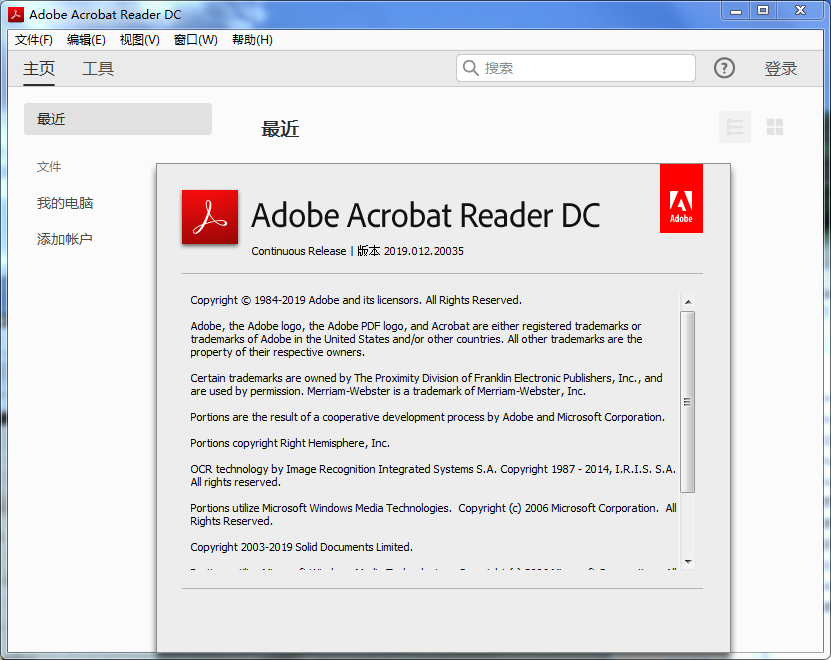
\includegraphics[width=0.9\textwidth]{01acrobat/01aboutacrobatreaderdc}
  \end{columns}
\end{frame}

\begin{frame}{PC计算机}{Acrobat Reader DC}
  \begin{columns}[T]
    \column{0.55\textwidth}
    \begin{itemize}
    \item 打开\enquote{注释}工具栏
      \begin{itemize}\itemsep=5pt%[itemsep=10pt]
      \item \menu{视图>工具>注释>打开}
      \item 工具边栏\keys{注释}图标
      \end{itemize}
    \end{itemize}
    \begin{center}
      % node[near start,circle,fill=black,,inner sep=0pt,minimum size=3pt,white] {\tiny 1}
      \begin{annotationimage}{width=0.9\textwidth}{01acrobat/02openreviewtools01}
        % 利用fit库绘制命名矩形
        \node[fit={(0.145,0.89) (0.235,0.96)}, inner sep=0pt, draw=red, thick] (view) {};
        \node[fit={(0.23,0.53) ($(0.23, 0.53) + (0.07, 0.045)$)}, inner sep=0pt, draw=red, thick] (tools) {};
        \node[fit={(0.522,0.52) ($(0.522, 0.52) + (0.05, 0.045)$)}, inner sep=0pt, draw=red, thick] (annotation) {};
        \node[fit={(0.755,0.52) ($(0.755, 0.52) + (0.075, 0.045)$)}, inner sep=0pt, draw=red, thick] (open) {};
        % 绘制箭头连线表示操作顺序
        \draw[-{Stealth[scale=0.8]}, blue, thick] (view.south) to
        [out=-90, in=180] node[midway,circle,fill=blue,inner sep=0pt,minimum size=3pt,text=yellow]
        {\scriptsize \sffamily 1}(tools.west);
        \draw[-{Stealth[scale=0.8]}, blue, thick] (tools.east) to [out=0, in=180]
        node[midway,circle,fill=blue,inner sep=0pt,minimum size=3pt,text=yellow]
        {\scriptsize \sffamily 2}(annotation.west);
        \draw[-{Stealth[scale=0.8]}, blue, thick] (annotation.east) to
        [out=0, in=180]node[midway,circle,fill=blue,inner sep=0pt,minimum size=3pt,text=yellow]
        {\scriptsize \sffamily 3}(open.west);
      \end{annotationimage}
    \end{center}
    \column{0.45\textwidth}
    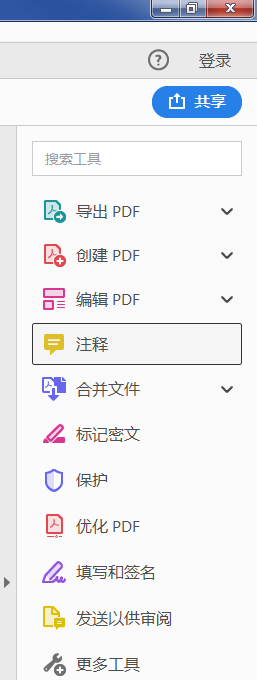
\includegraphics[height=0.8\textheight]{01acrobat/03openreviewtools02}\qquad
    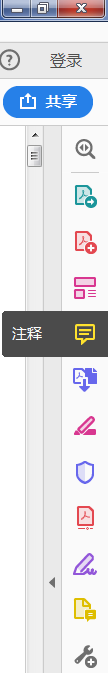
\includegraphics[height=0.8\textheight]{01acrobat/03openreviewtools03}
  \end{columns}
\end{frame}

\begin{frame}{PC计算机}{Acrobat Reader DC}
  \begin{itemize}
  \item \enquote{注释}工具栏
    \begin{itemize}
    \item 用于添加各类注释
    \end{itemize}
  \end{itemize}
  \begin{center}
    \begin{annotationimage}{width=0.8\textwidth}{01acrobat/03openreviewtools04}
        % 利用fit库绘制命名矩形
        \node[fit={(0.285,0.81) (0.72, 0.85)}, inner sep=0pt, draw=red, thick] (tools) {};
        % 绘制说明标记
        \node (annotation) [red,right=of tools,shift={(-0.06, -0.15)}] {\small \enquote{注释}工具栏};
        % 绘制箭头连线表示操作顺序
        \draw[-{Stealth[scale=0.8]}, blue, thick] (annotation.north) to [out=90, in=0] (tools.east);
      \end{annotationimage}
  \end{center}
\end{frame}

\begin{frame}{PC计算机}{Acrobat Reader DC}
  \begin{itemize}
  \item \enquote{注释}工具栏
    \begin{itemize}
    \item \enquote{批注}工具
    \end{itemize}
  \end{itemize}
  
  \begin{center}
    \begin{annotationimage}{width=0.8\textwidth}{01acrobat/03reviewicons01}
      % 绘制外观设置按钮分组示意下划线
      \draw[thick,blue] (0.86,0.26) -- (1.0,0.26);
      % 添加各图标标注
      \foreach \ann/\xpos in
      {
        {附\\注\\工\\具}/0.02, {高\\亮\\工\\具}/0.07,
        {下\\划\\线\\工\\具}/0.126, {删\\除\\线\\工\\具}/0.18,
        {删\\除\\线\\并\\插\\入\\附\\注\\工\\具}/0.229, {插\\入\\文\\本\\工\\具}/0.283,
        {文\\本\\工\\具}/0.346, {文\\本\\框\\工\\具}/0.40,
        {铅\\笔\\绘\\图\\工\\具}/0.45, {铅\\笔\\擦\\工\\具}/0.51,
        {图\\章\\工\\具}/0.56, {附\\加\\文\\件\\工\\具}/0.63,
        {绘\\图\\工\\具}/0.7, {保\\持\\选\\择\\工\\具}/0.79,
        {注\\释\\外\\观\\设\\置}/0.93
      }
      {
        \draw[annotation below = {{\ann} at \xpos}] to (\xpos,0.48);
      }
      % \draw[annotation below = {附\\注\\工\\具 at 0.02}] to (0.02,0.5);
      % \draw[annotation below = {高\\亮\\工\\具 at 0.07}] to (0.07,0.5);
      % \draw[annotation below = {下\\划\\线\\工\\具 at 0.126}] to (0.126,0.5);
      % \draw[annotation below = {删\\除\\线\\工\\具 at 0.18}] to (0.18,0.5);
      % \draw[annotation below = {删\\除\\附\\注\\工\\具 at 0.229}] to (0.229,0.5);
      % \draw[annotation below = {插\\入\\文\\本\\工\\具 at 0.283}] to (0.283,0.5);
      % \draw[annotation below = {文\\本\\工\\具 at 0.346}] to (0.346,0.5);
      % \draw[annotation below = {文\\本\\框\\工\\具 at 0.40}] to (0.40,0.5);
      % \draw[annotation below = {铅\\笔\\绘\\图\\工\\具 at 0.45}] to (0.45,0.5);
      % \draw[annotation below = {铅\\笔\\擦\\工\\具 at 0.51}] to (0.51,0.5);
      % \draw[annotation below = {图\\章\\工\\具 at 0.56}] to (0.56,0.5);
      % \draw[annotation below = {附\\加\\文\\件\\工\\具 at 0.63}] to (0.63,0.5);
      % \draw[annotation below = {绘\\图\\工\\具 at 0.7}] to (0.7,0.5);
      % \draw[annotation below = {保\\持\\选\\择\\工\\具 at 0.79}] to (0.79,0.5);
      % \draw[thick,blue] (0.86,0.28) -- (1.0,0.28);
      % \draw[annotation below = {注\\释\\外\\观\\设\\置 at 0.93}] to (0.93,0.5); 
      % 附注工具、高亮工具、下划线工具、删除线工具、删除附注工具、插入
      % 文本工具、文本注释工具、文本框工具、铅笔工具、铅笔橡皮擦工具、图章工具、附
      % 加文件、绘图工具、保持选择工具、注释的外观工具
    \end{annotationimage}
  \end{center}
\end{frame}

\begin{frame}{PC计算机}{Acrobat Reader DC}
  \begin{itemize}
  \item 使用\enquote{批注}工具添加注释
    \begin{itemize}
    \item 详见:\link{https://helpx.adobe.com/cn/acrobat/using/commenting-pdfs.html}
    \end{itemize}
  \end{itemize}
  
  \begin{center}
    \begin{annotationimage}{width=0.55\textwidth}{01acrobat/04adddeleteline}      
    \end{annotationimage}
    \begin{annotationimage}{width=0.55\textwidth}{01acrobat/04addtextbox}      
    \end{annotationimage}
  \end{center}
\end{frame}

\begin{frame}{PC计算机}{Acrobat Reader DC}
  \begin{columns}[t]
    \column{0.35\textwidth}
    \begin{itemize}
    \item 管理注释
      \begin{itemize}\itemsep=10pt
      \item 复制
      \item 编辑
      \item 删除
      \item 设置状态
      \item 属性
      \item 添加勾形
      \end{itemize}
    \end{itemize}
    \column{0.45\textwidth}
    \begin{center}
      \begin{annotationimage}{height=0.75\textheight}{01acrobat/04editreviewcontents}
      \end{annotationimage}
    \end{center}
  \end{columns}
\end{frame}

\subsection{Foxit福昕}
\begin{frame}{PC计算机}{Foxit福昕}
  \begin{columns}[c]
    \column{0.35\textwidth}
    \begin{itemize}
    \item 基本功能
      \begin{itemize}
      \item 查看、打印PDF文档
      \item \alert{注释}PDF文档
      \item 其它
      \end{itemize}
    \item 适用平台
      \begin{itemize}
      \item Windows
      \item Mac OS
      \item Linux
      \item Android
      \item iOS
      \end{itemize}
    \item 下载链接
      \begin{itemize}
      \item 官网\link{https://www.foxitsoftware.cn/downloads/}
      \end{itemize}
    \item 授权
      \begin{itemize}
      \item \alert{免费}
      \end{itemize}
    \end{itemize}
    \column{0.55\textwidth}
    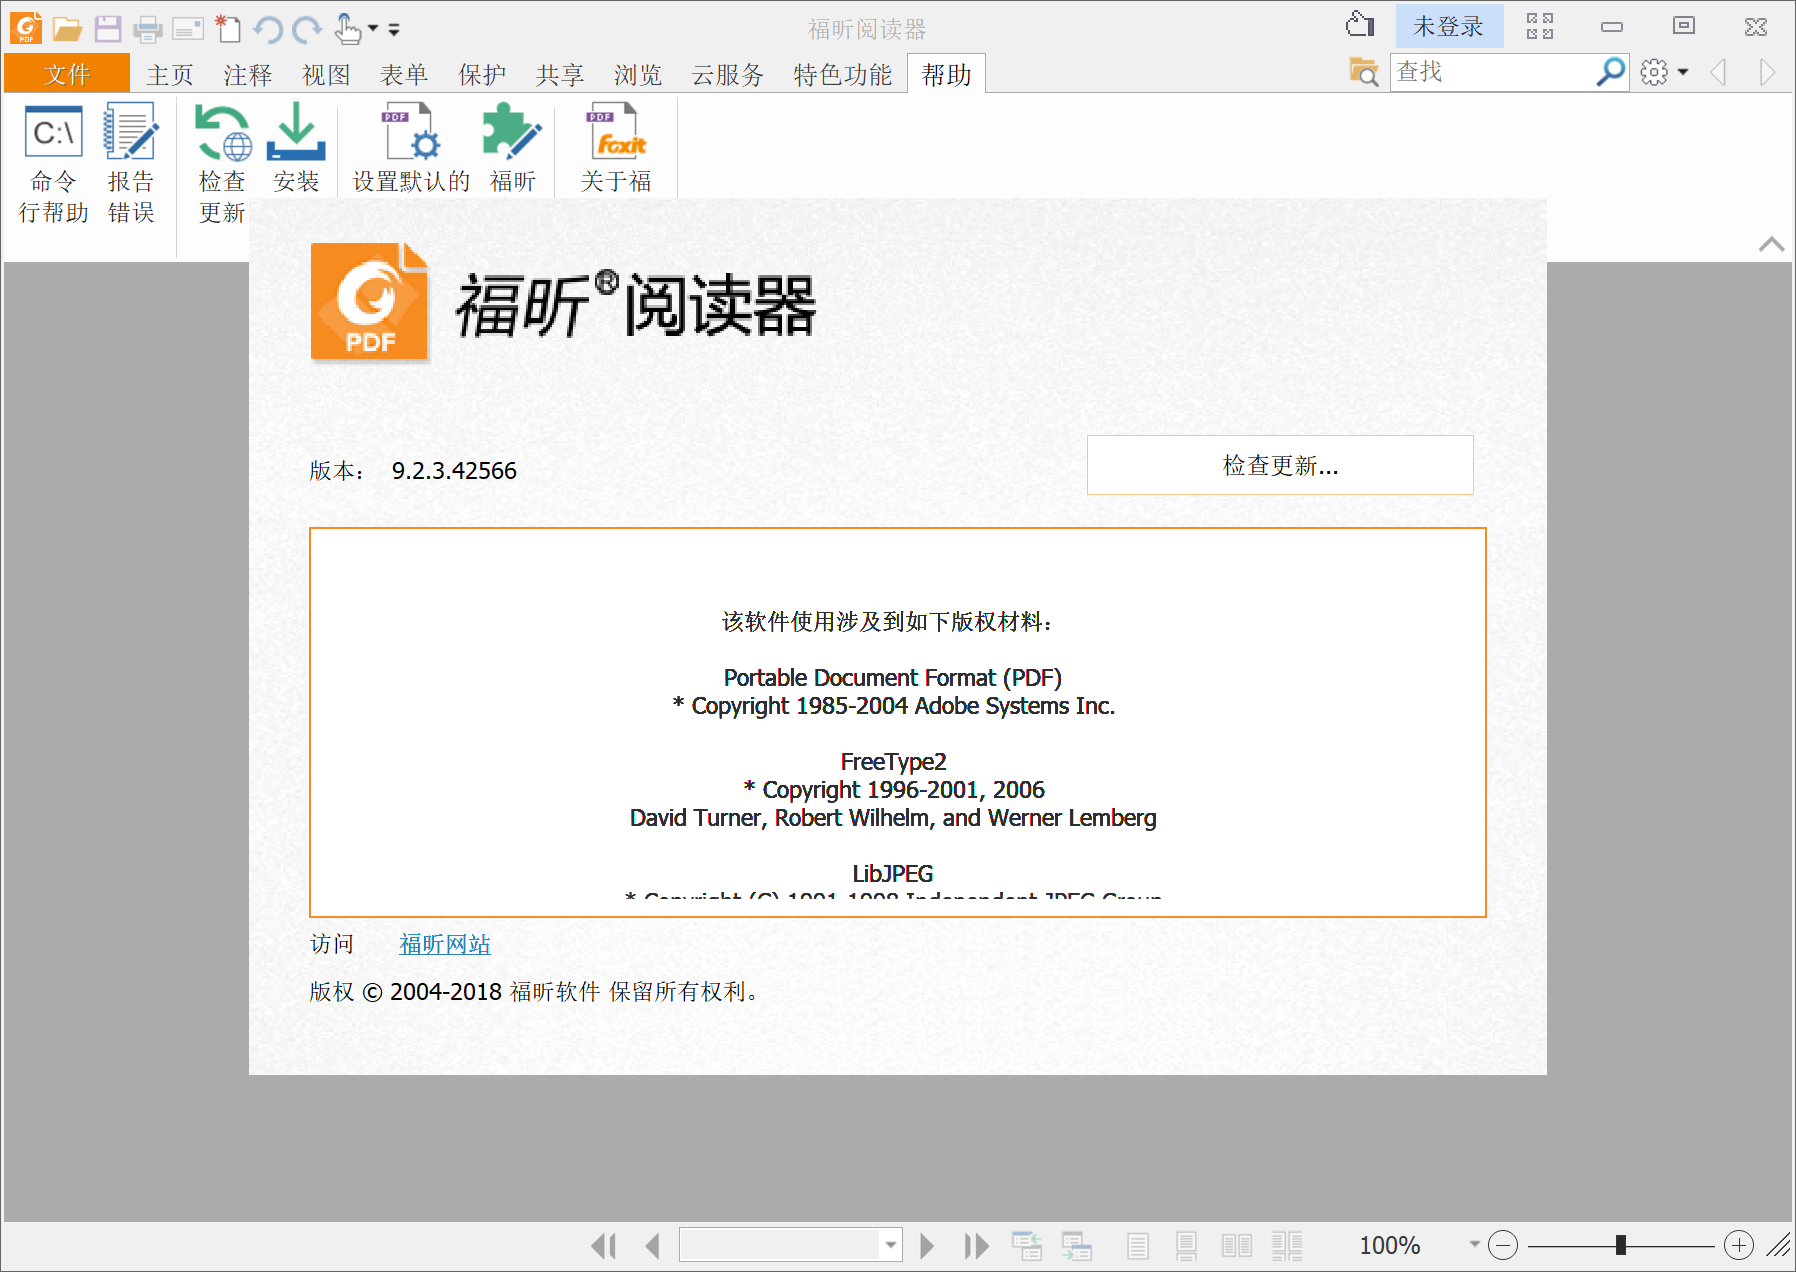
\includegraphics[width=1.0\textwidth]{02foxitreader/01foxitabout}
  \end{columns}
\end{frame}

\begin{frame}{PC计算机}{Foxit福昕}
  \begin{itemize}
  \item \enquote{注释}工具栏
    \begin{itemize}
    \item \menu{注释}菜单打开\enquote{注释}工具栏
    \end{itemize}
  \end{itemize}
  \begin{center}
    \begin{annotationimage}{width=0.9\textwidth}{02foxitreader/03foxitanntoolbar}
    \end{annotationimage}
  \end{center}
\end{frame}

\begin{frame}{PC计算机}{Foxit福昕}
  \begin{itemize}
  \item \enquote{注释}工具栏
    \begin{itemize}
    \item 添加各类\enquote{注释}\footnote[frame,1]{与Acrobat Reader DC
        软件操作基本一致。}
    \item 管理各类\enquote{注释}
    \end{itemize}
  \end{itemize}
  \begin{center}
    \begin{annotationimage}{width=0.5\textwidth}{02foxitreader/02foxitgui}
    \end{annotationimage}
  \end{center}
\end{frame}


\subsection{金山PDF}
\begin{frame}{PC计算机}{金山PDF}
  \begin{columns}[c]
    \column{0.35\textwidth}
    \begin{itemize}
    \item 基本功能
      \begin{itemize}
      \item 查看、打印PDF文档
      \item \alert{注释}PDF文档
      \item 其它
      \end{itemize}
    \item 适用平台
      \begin{itemize}
      \item Windows
      \item 其它平台未知
      \end{itemize}
    \item 下载链接
      \begin{itemize}
      \item 官网\link{https://www.wps.cn/product/kingsoftpdf/}
      \end{itemize}
    \item 授权
      \begin{itemize}
      \item \alert{免费}
      \end{itemize}
    \end{itemize}
    \column{0.55\textwidth}
    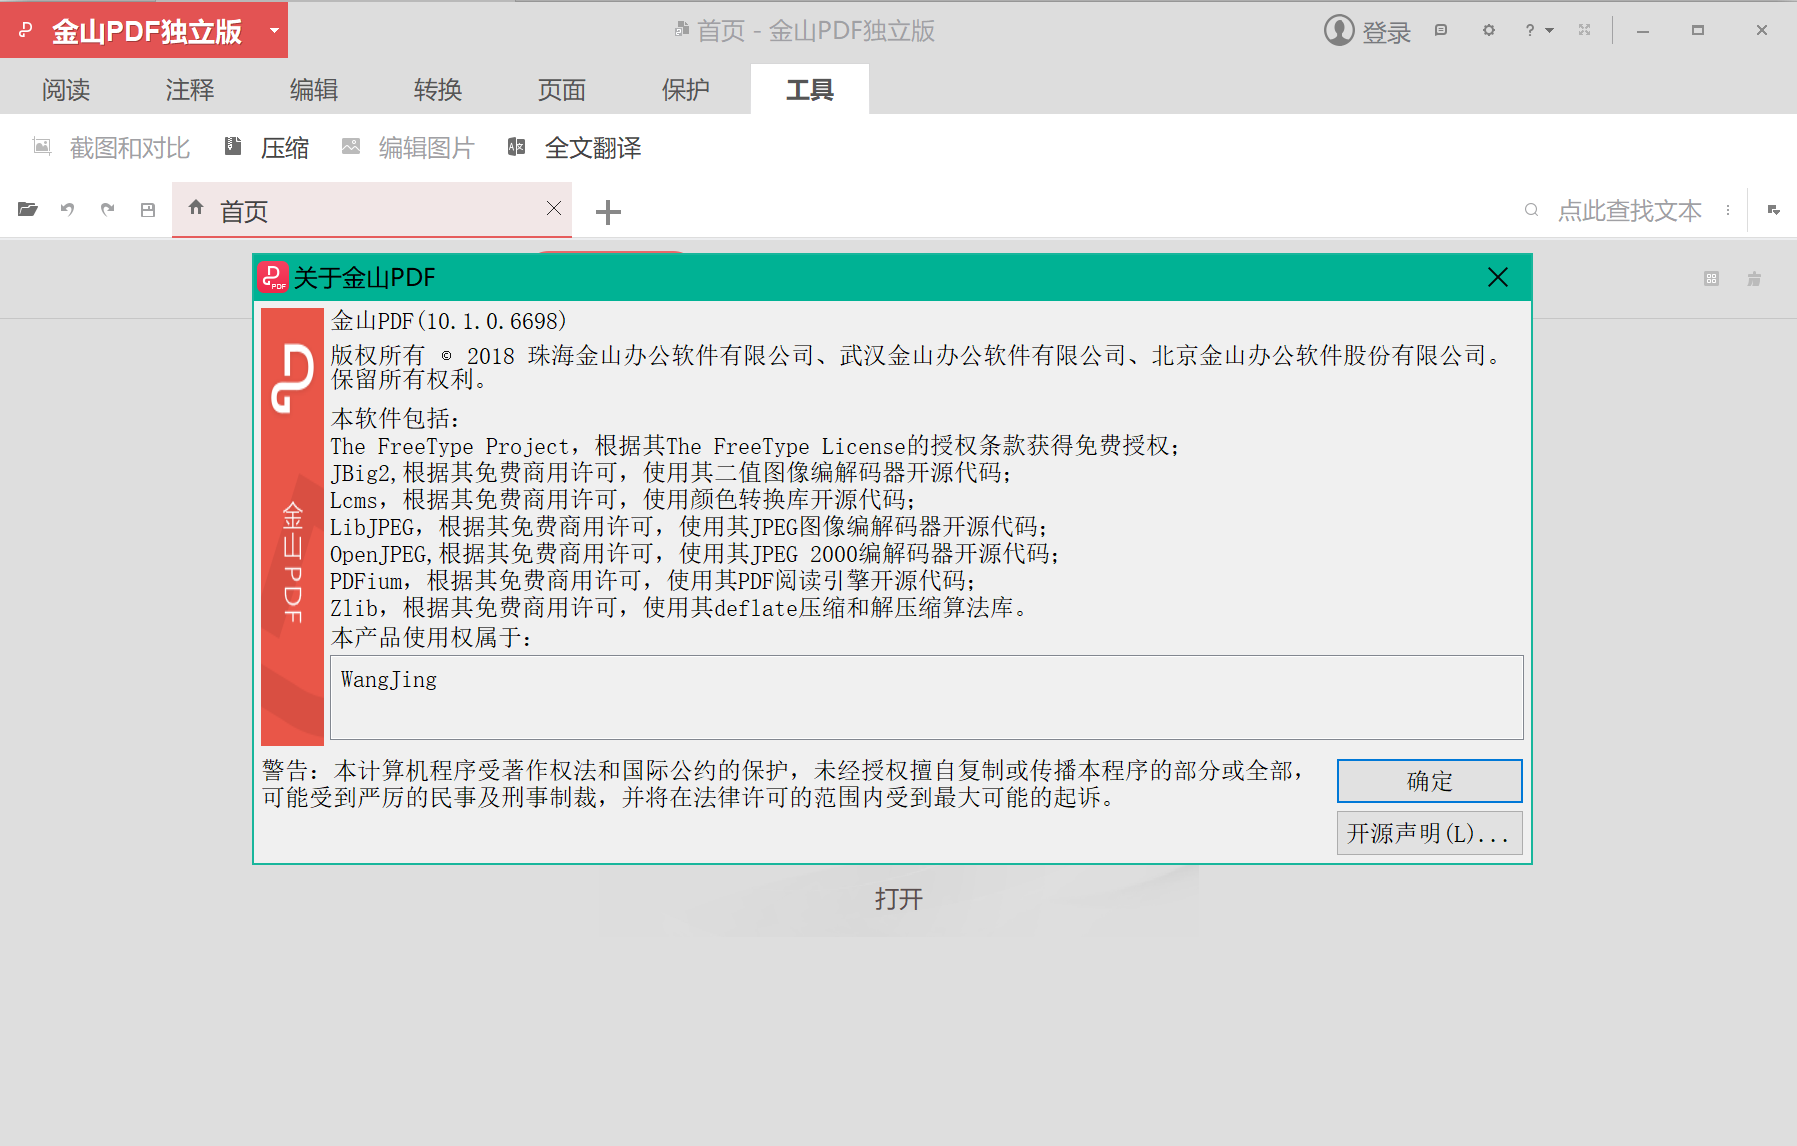
\includegraphics[width=1.0\textwidth]{03kingsoftpdf/01kingsoftpdfabout}
  \end{columns}
\end{frame}

\begin{frame}{PC计算机}{金山PDF}
  \begin{itemize}
  \item \enquote{注释}工具栏
    \begin{itemize}
    \item \menu{注释}菜单打开\enquote{注释}工具栏
    \end{itemize}
  \end{itemize}
  \begin{center}
    \begin{annotationimage}{width=0.9\textwidth}{03kingsoftpdf/03kingsoftpdfanntoolbar}
    \end{annotationimage}
  \end{center}
\end{frame}

\begin{frame}{PC计算机}{金山PDF}
  \begin{itemize}
  \item \enquote{注释}工具栏
    \begin{itemize}
    \item 添加各类\enquote{注释}\footnote[frame,1]{与Acrobat Reader DC
        软件操作基本一致。}
    \item 管理各类\enquote{注释}\footnote[frame,2]{注意使用
        \enquote{\alert{超级注释模式}}。}
    \end{itemize}
  \end{itemize}
  \begin{center}
    \begin{annotationimage}{width=0.5\textwidth}{03kingsoftpdf/042kingsoftpdfsuper}
    \end{annotationimage}
  \end{center}
\end{frame}

\subsection{Okular}
\begin{frame}{PC计算机}{Okular}
  \begin{columns}[c]
    \column{0.35\textwidth}
    \begin{itemize}
    \item 基本功能
      \begin{itemize}
      \item 查看、打印PDF文档
      \item \alert{注释}PDF文档
      \item 其它
      \end{itemize}
    \item 适用平台
      \begin{itemize}
      \item Windows
      \item Mac OS
      \item Linux
      \end{itemize}
    \item 下载链接
      \begin{itemize}
      \item 官网
        \link{https://okular.kde.org/}\footnote[frame,1]{Ubuntu平台可
          以直接使用:sudo apt install okular命令进行安装。}
      \end{itemize}
    \item 授权
      \begin{itemize}
      \item \alert{免费}
      \end{itemize}
    \end{itemize}
    \column{0.55\textwidth}
    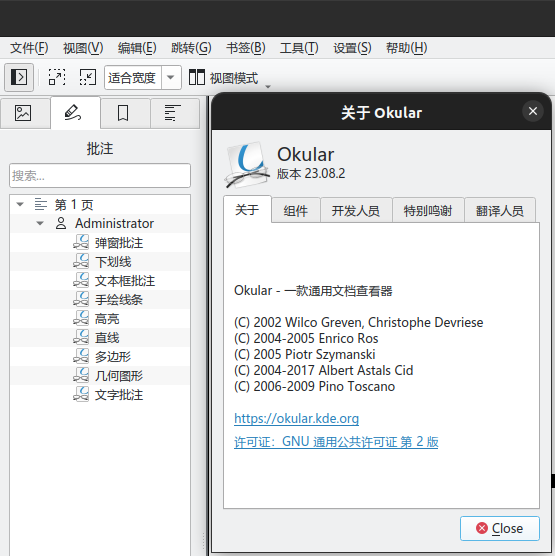
\includegraphics[width=0.95\textwidth]{04okular/01okularabout}
  \end{columns}
\end{frame}

\begin{frame}{PC计算机}{Okular}
  \begin{itemize}
  \item \enquote{注释}工具栏
    \begin{itemize}
    \item \menu{注释}菜单打开\enquote{注释}工具栏
    \end{itemize}
  \end{itemize}
  \begin{center}
    \begin{annotationimage}{height=0.7\textheight}{04okular/03okulartoolbar}
    \end{annotationimage}
  \end{center}
\end{frame}

\begin{frame}{PC计算机}{Okular}
  \begin{itemize}
  \item \enquote{注释}工具栏
    \begin{itemize}
    \item 添加各类\enquote{注释}\footnote[frame,1]{与Acrobat Reader DC
        软件操作基本一致。}
    \item 管理各类\enquote{注释}
    \end{itemize}
  \end{itemize}
  \begin{center}
    \begin{annotationimage}{width=0.6\textwidth}{04okular/02okulargui}
    \end{annotationimage}
  \end{center}
\end{frame}

\subsection{Xournal++}

\begin{frame}{PC计算机}{Xournal++}
  \begin{columns}[c]
    \column{0.35\textwidth}
    \begin{itemize}
    \item 基本功能
      \begin{itemize}
      \item 手写笔记
      \item \alert{标注}PDF文档
      \item 其它
      \end{itemize}
    \item 适用平台
      \begin{itemize}
      \item Windows
      \item Mac OS
      \item Linux
      \end{itemize}
    \item 下载链接
      \begin{itemize}
      \item 官网
        \link{https://xournalpp.github.io/}
      \end{itemize}
    \item 授权
      \begin{itemize}
      \item \alert{免费}
      \end{itemize}
    \end{itemize}
    \column{0.55\textwidth}
    \vspace{1ex}
    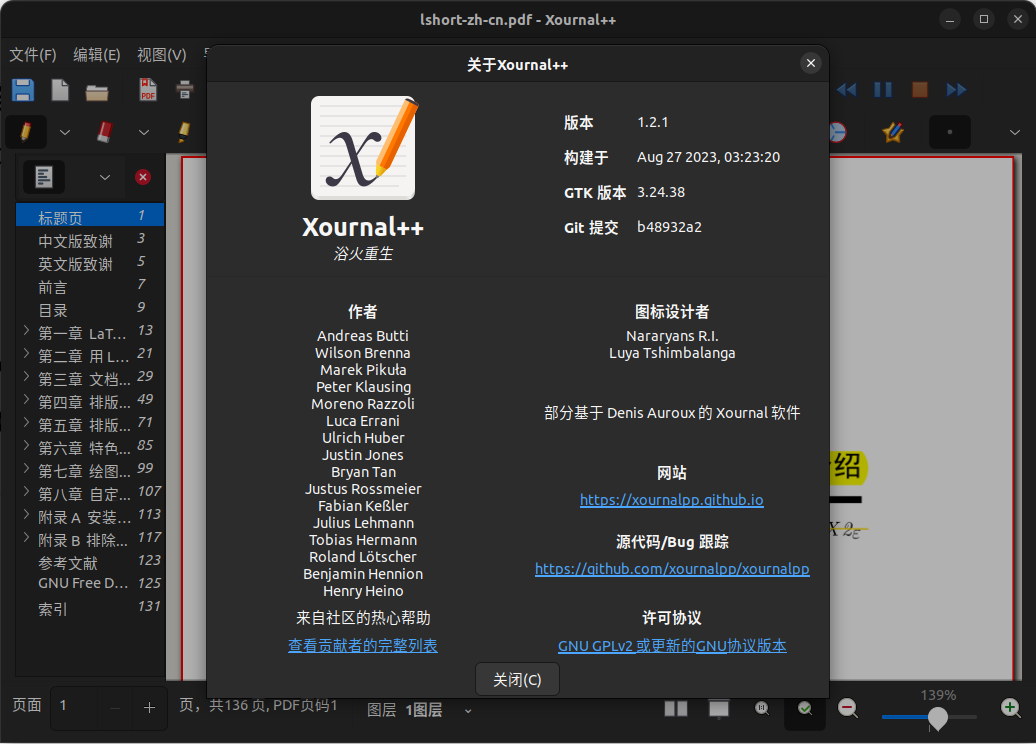
\includegraphics[width=0.85\textwidth]{08xournal++/01xournalabout}
  \end{columns}
\end{frame}

\begin{frame}{PC计算机}{Xournal++}
  \begin{itemize}
  \item \enquote{标注}工具栏
  \end{itemize}
  \vspace{3ex}
  \begin{center}
      \begin{annotationimage}{width=0.95\textwidth}{08xournal++/02xournaltoolbar}
      % 绘制外观设置按钮分组示意下划线
      \draw[thick,blue] (0.52,0.20) -- (0.59,0.20);
      \draw[thick,blue] (0.65,0.20) -- (1.00,0.20);
      % 添加各图标标注
      \foreach \ann/\xpos in
      {
        {画\\笔\\工\\具}/0.018,
        {橡\\皮\\工\\具}/0.070,
        {高\\亮\\工\\具}/0.124,
        {插\\入\\图\\像}/0.155,
        {插\\入\\文\\本}/0.182,
        {插\\入\\公\\式}/0.210,
        {插\\入\\图\\形}/0.255,
        {旋\\转\\吸\\附}/0.302,
        {网\\格\\截\\图}/0.330,
        {填\\充\\图\\形}/0.385,
        {垂\\直\\间\\距}/0.422,
        {移\\动\\对\\象}/0.453,
        {缺\\省\\工\\具}/0.490,
        {画\\笔\\宽\\度}/0.556,
        {填\\充\\工\\具}/0.625,
        {画\\笔\\颜\\色}/0.820
      }
      {
        \draw[annotation below = {{\ann} at \xpos}] to (\xpos,0.48);
      }
    \end{annotationimage}
    % 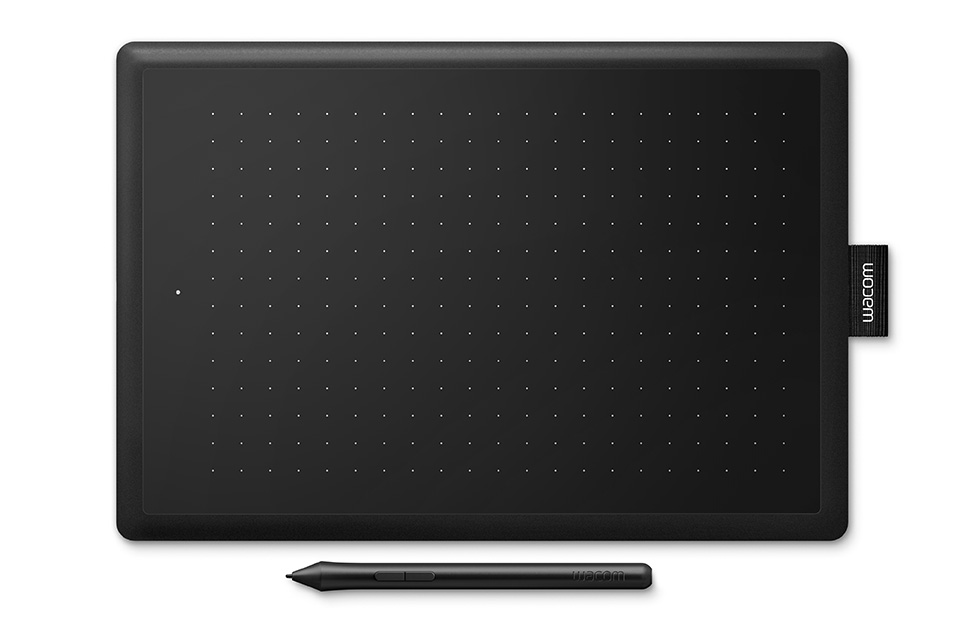
\includegraphics[width=0.40\textwidth]{08xournal++/04wacom}
  \end{center}
\end{frame}

\begin{frame}{PC计算机}{Xournal++}
  \begin{itemize}
  \item 手写与\enquote{标注}
  \end{itemize}
  \vspace{2ex}
  \begin{columns}[c]
    \column{0.75\textwidth}
    \centering
    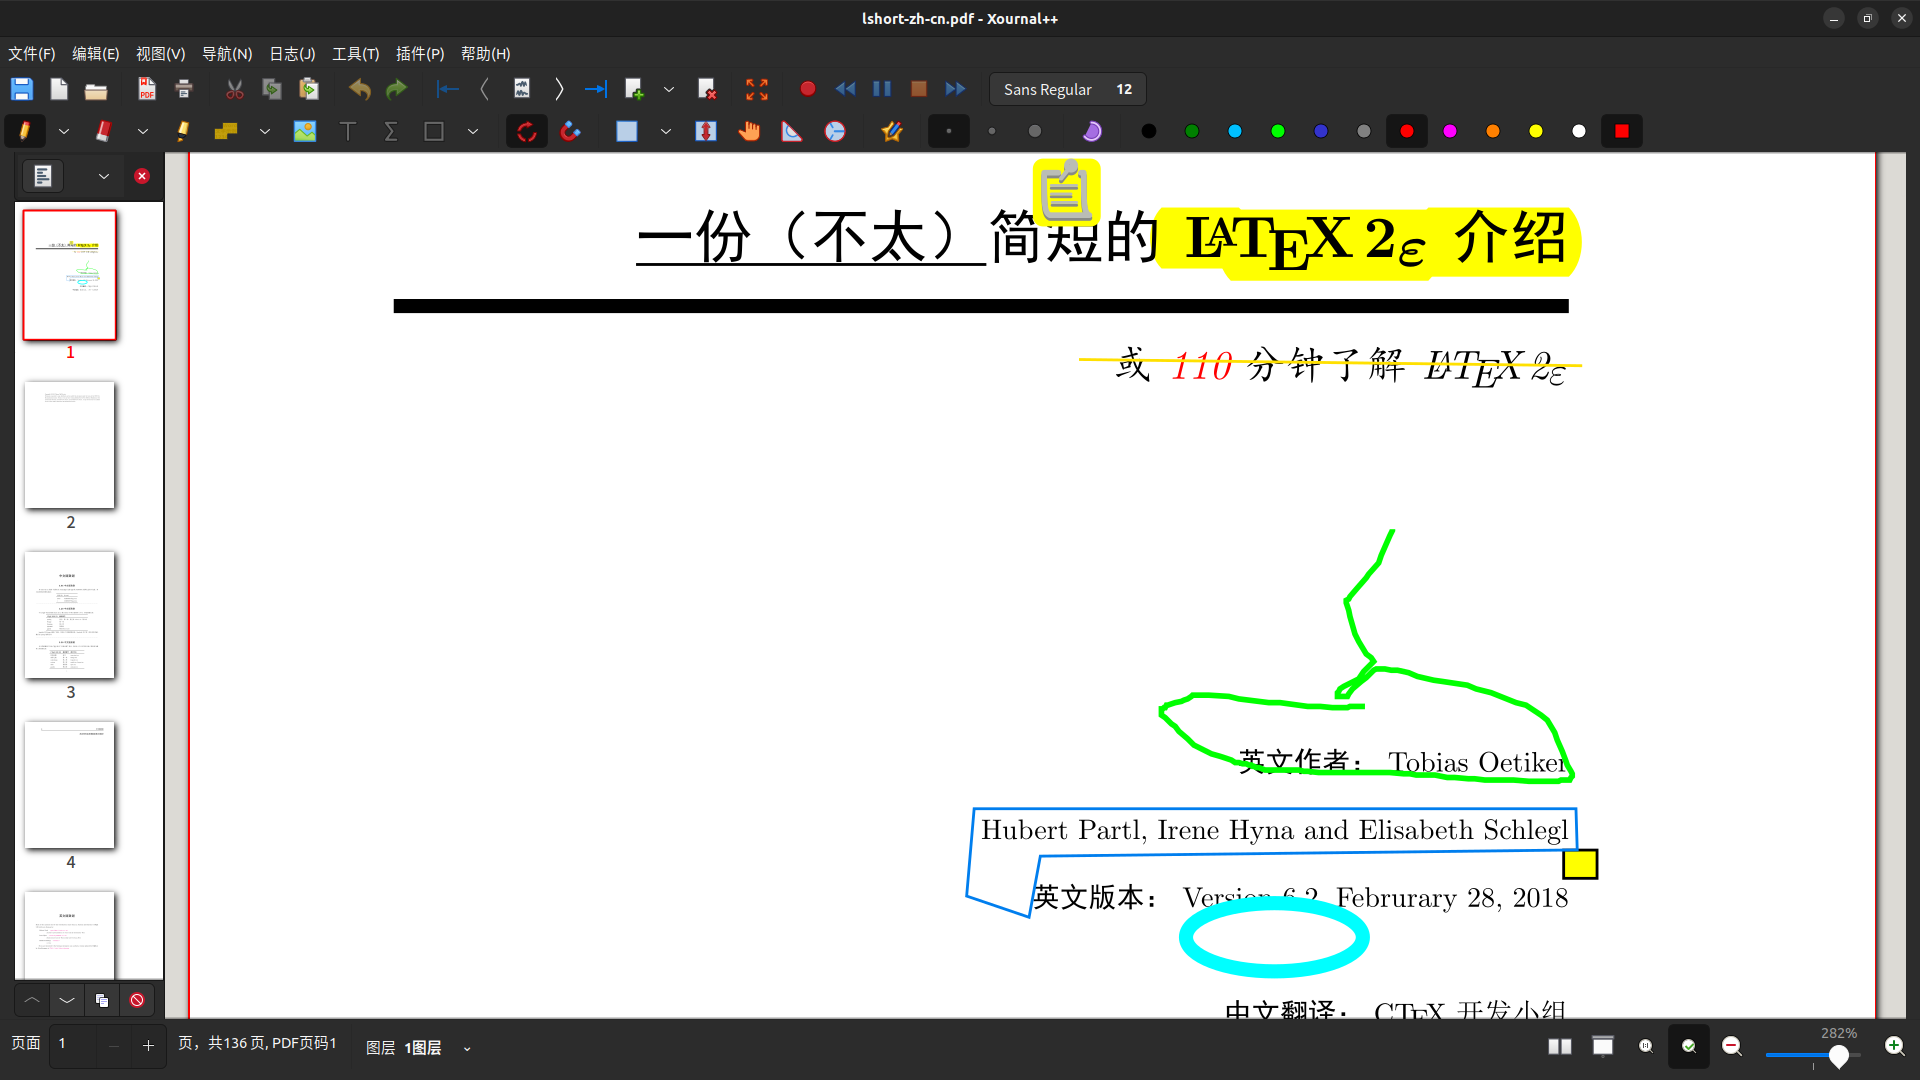
\includegraphics[width=0.90\textwidth]{08xournal++/03xournalex01}
    \column{0.25\textwidth}
    \centering
    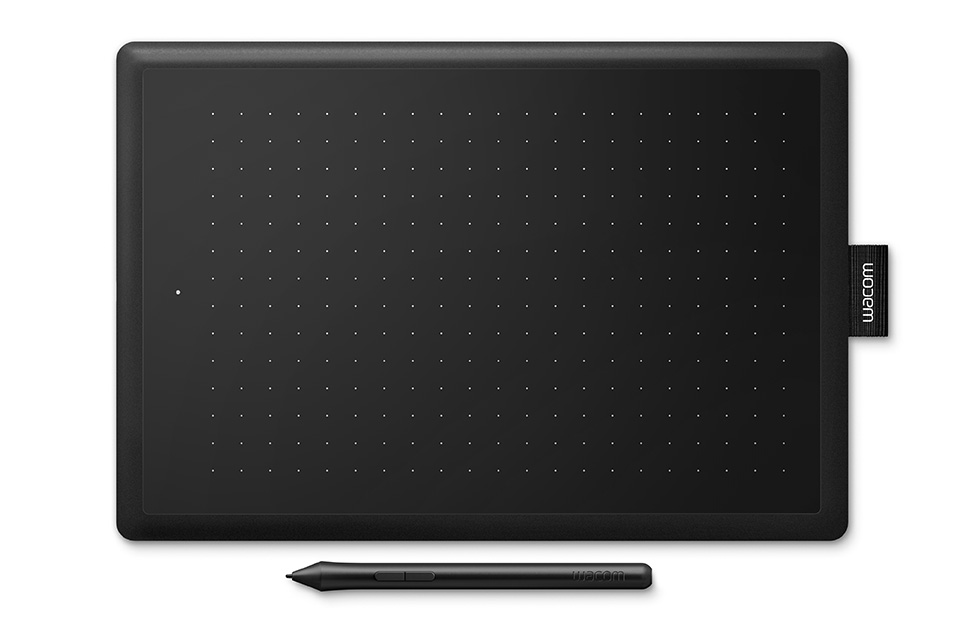
\includegraphics[width=1.00\textwidth]{08xournal++/04wacom}
  \end{columns}
\end{frame}

\begin{frame}[standout,plain]
  说明:\\
  软件其他功能也很强大\\
  只要\alert{熟悉一个软件}就好\\
  \alert{推荐}使用\enquote{Acrobat Reader DC},毕竟是\alert{原生的}\\
  肯定还有你偏好的其它软件
\end{frame}
\section{iOS平板}
\subsection{Goodnotes}
\begin{frame}{iOS平板}{Goodnotes}
  \begin{columns}[c]
    \column{0.45\textwidth}
    \begin{itemize}\itemsep=3pt
    \item 基本功能
      \begin{itemize}
      \item 笔记软件
      \item 支持Apple Pencil
      \item 可以\alert{批注}PDF文档
      \item 具备文字识别功能(OCR)
      \end{itemize}
    \item 适用平台
      \begin{itemize}
      \item iOS平板
      \item 其它平台未知
      \end{itemize}
    \item 下载链接
      \begin{itemize}
      \item Apple Store
      \end{itemize}
    \item 授权
      \begin{itemize}
      \item \alert{50.00RMB}
      \end{itemize}
    \end{itemize}
    \column{0.45\textwidth}
    
\includegraphics[height=0.75\textheight]{05goodnotes/01appstore}
  \end{columns}
\end{frame}

\begin{frame}{iOS平板}{Goodnotes}
  \begin{itemize}\itemsep=3pt
  \item 文件管理
    \begin{itemize}
    \item 创建文件夹
    \item 分门别类管理
    \end{itemize}
  \end{itemize}
  \begin{center}
    \begin{tikzpicture}
      \node[anchor=south west, inner sep=0](img1) at (0,0)
      {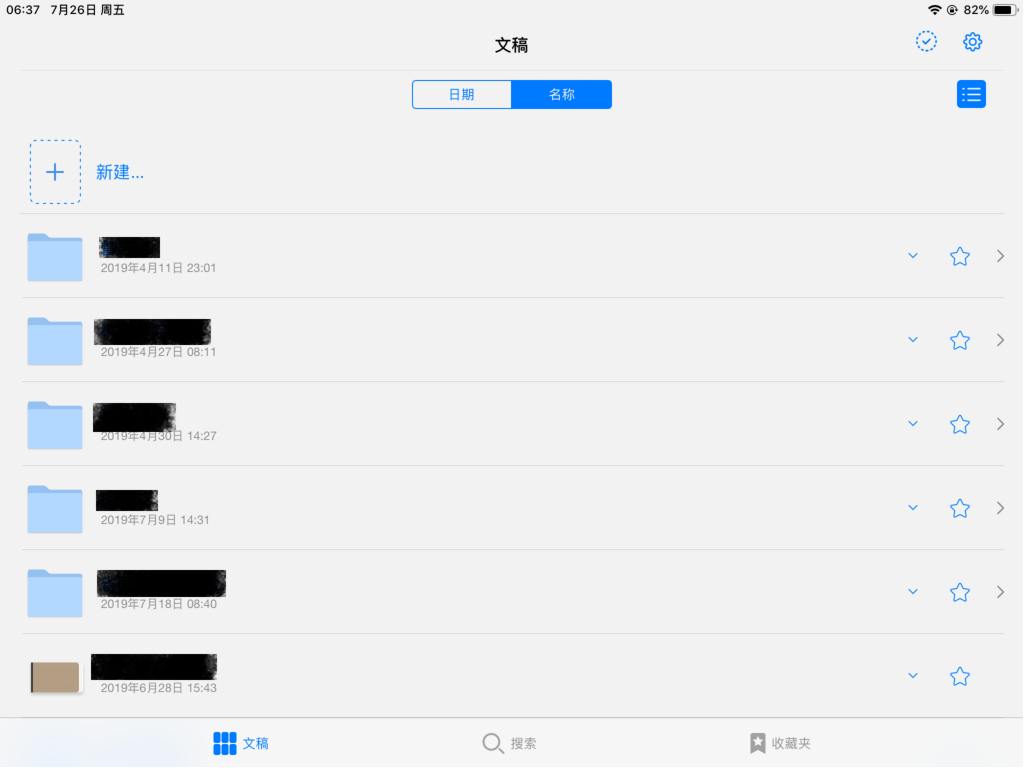
\includegraphics[width=0.34\textwidth]{05goodnotes/02gui01}};
      \node[anchor=south west, inner sep=0, right=0.1 of img1](img2) 
      {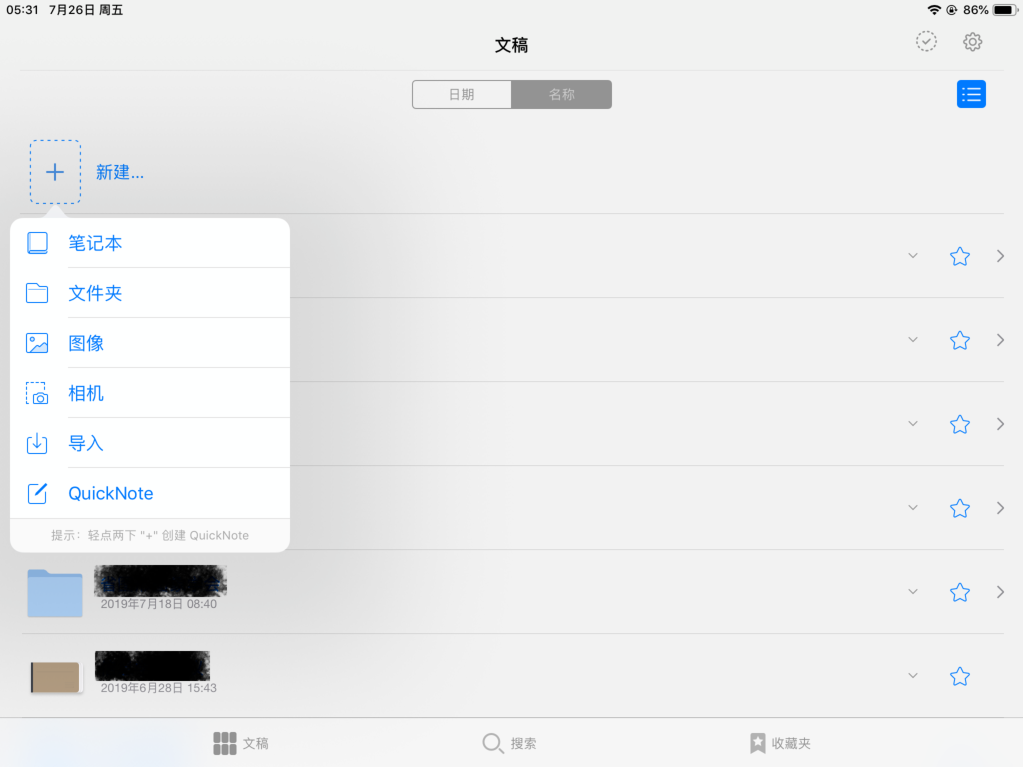
\includegraphics[width=0.34\textwidth]{05goodnotes/02gui02}};
      \node[anchor=south west, inner sep=0, right=0.1 of img2](img3)
      {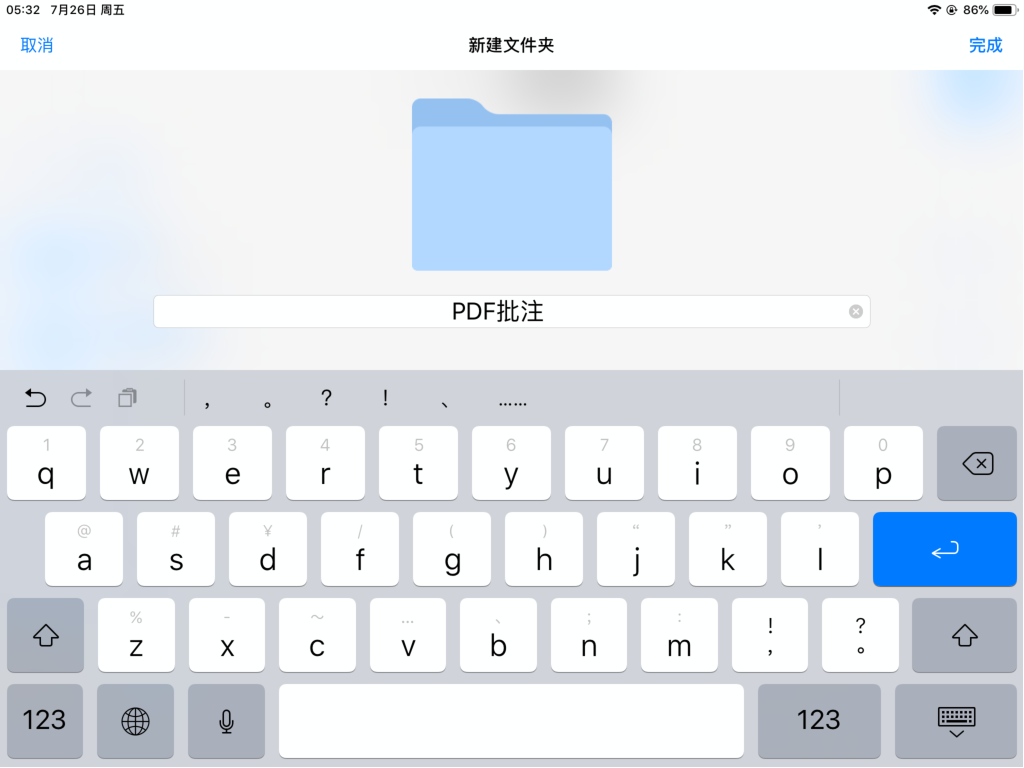
\includegraphics[width=0.34\textwidth]{05goodnotes/03creatfold}};

      \begin{scope}[x={(img3.south east)},y={(img1.north west)}]
        % 绘制坐标辅助网络
        % \draw[very thin, draw=\finegridcolor, step=0.02] (0,0) grid (1,1);
        % \draw[thin, draw=\maingridcolor, xstep=0.1, ystep=0.1] (0,0) grid (1,1);
        % \foreach \x in {0,1,...,9} {
        %   \node [anchor=north] at (\x/10,0) {\tiny 0.\x};
        % }
        % \node [anchor=north] at (1,0) {\tiny 1};

        % \foreach \y in {0,1,...,9} {
        %   \node [anchor=east] at (0,\y/10) {\tiny 0.\y};
        % }
        % \node [anchor=east] at (0,1) {\tiny 1};
        
        % 利用fit库绘制命名矩形
        \node[fit={(0.008,0.731) (0.046, 0.825)}, inner sep=0pt, draw=red, thick] (new) {};
        \node[fit={(0.340,0.590) (0.379, 0.644)}, inner sep=0pt, draw=red, thick] (fold) {};
        \node[fit={(0.805,0.570) (0.868, 0.617)}, inner sep=0pt, draw=red, thick] (name) {};
        % 绘制箭头连线表示操作顺序
        \draw[-{Stealth[scale=0.8]}, red, thick] (new.east) to [out=0,
        in=180] node[midway,circle,fill=black,inner sep=0pt,minimum
        size=3pt,text=white] {\scriptsize \sffamily 1}(fold.west);
        \draw[-{Stealth[scale=0.8]}, red, thick] (fold.east) to
        [out=0, in=180]node[midway,circle,fill=black,inner
        sep=0pt,minimum size=3pt,text=white] {\scriptsize \sffamily 2}
        (name.west);
      \end{scope}
    \end{tikzpicture}
  \end{center}
\end{frame}

\begin{frame}{iOS平板}{Goodnotes}
  \begin{itemize}\itemsep=3pt
  \item 导入PDF文件
    \begin{itemize}
    \item 进入\enquote{PDF批注}文件夹
    \item 从\enquote{iCloud云盘}导入
    \end{itemize}
  \end{itemize}
  \begin{center}
    \begin{tikzpicture}
      \node[anchor=south west, inner sep=0](img1) at (0,0)
      {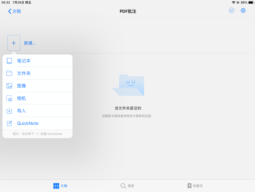
\includegraphics[width=0.45\textwidth]{05goodnotes/04importmenu}};
      \node[anchor=south west, inner sep=0, right=0.1 of img1](img2) 
      {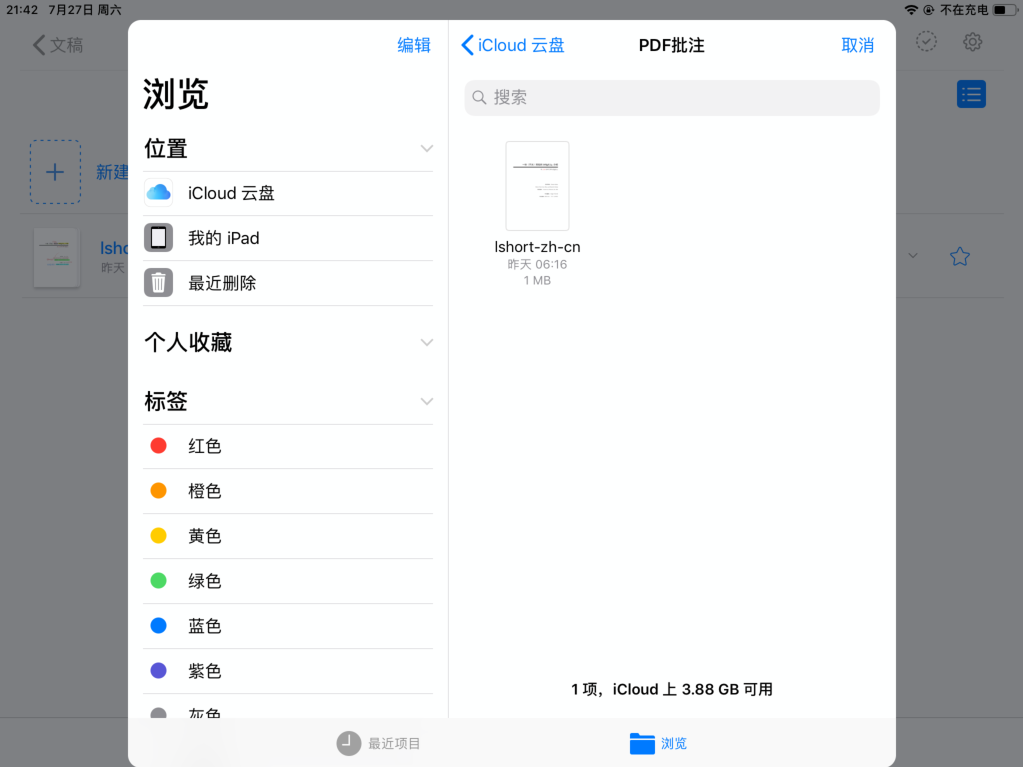
\includegraphics[width=0.45\textwidth]{05goodnotes/05importicloud}};

      \begin{scope}[x={(img2.south east)},y={(img1.north west)}]
        % 绘制坐标辅助网络
        % \draw[very thin, draw=\finegridcolor, step=0.02] (0,0) grid (1,1);
        % \draw[thin, draw=\maingridcolor, xstep=0.1, ystep=0.1] (0,0) grid (1,1);
        % \foreach \x in {0,1,...,9} {
        %   \node [anchor=north] at (\x/10,0) {\tiny 0.\x};
        % }
        % \node [anchor=north] at (1,0) {\tiny 1};

        % \foreach \y in {0,1,...,9} {
        %   \node [anchor=east] at (0,\y/10) {\tiny 0.\y};
        % }
        % \node [anchor=east] at (0,1) {\tiny 1};

        % 利用fit库绘制命名矩形
        \node[fit={(0.23,0.92) (0.268, 0.96)}, inner sep=0pt, draw=blue, thick] (pdffold) {};

        \node[fit={(0.008,0.731) (0.073, 0.825)}, inner sep=0pt, draw=red, thick] (new) {};
        \node[fit={(0.008,0.4) (0.055, 0.445)}, inner sep=0pt, draw=red, thick] (import) {};
        \node[fit={(0.57,0.73) (0.66, 0.77)}, inner sep=0pt, draw=red, thick] (icloud) {};
        \node[fit={(0.69,0.92) (0.78, 0.96)}, inner sep=0pt, draw=blue, thick] (icloudroot) {};
        \node[fit={(0.81,0.92) (0.85, 0.96)}, inner sep=0pt, draw=blue, thick] (icloudpdf) {};
        \node[fit={(0.74,0.62) (0.79, 0.83)}, inner sep=0pt, draw=red, thick] (pdfname) {};
        % 绘制箭头连线表示操作顺序
        \draw[-{Stealth[scale=0.8]}, blue, thick] (pdffold.west) to
        [out=180, in=90] (new.north);
        
        \draw[-{Stealth[scale=0.8]}, red, thick] (new.east) to [out=0,
        in=180] node[midway,circle,inner sep=0pt,minimum
        size=3pt,text=white,fill=black] {\scriptsize \sffamily 1}(import.west);
        
        
        \draw[-{Stealth[scale=0.8]}, red, thick] (import.east) to
        [out=0, in=180] node[midway,circle,inner
        sep=0pt,minimum size=3pt,text=white,fill=black] {\scriptsize \sffamily
          2}(icloud.west);
        
        
        \draw[-{Stealth[scale=0.8]}, red, thick] (icloud.east) to
        [out=0, in=180]node[midway,circle,fill=black,inner
        sep=0pt,minimum size=3pt,text=white,fill=black] {\scriptsize \sffamily 3} (pdfname.west);
        
        \draw[-{Stealth[scale=0.8]}, blue, thick] (icloudroot.east) to
        [out=0, in=180] (icloudpdf.west);
        
        \draw[-{Stealth[scale=0.8]}, blue, thick] (icloudpdf.south) to
        [out=-90, in=45] (pdfname.north);
        
      \end{scope}
    \end{tikzpicture}
  \end{center}
\end{frame}

\begin{frame}{iOS平板}{Goodnotes}
  \begin{itemize}\itemsep=3pt
  \item 导入PDF文件
    \begin{itemize}
    \item 进入\enquote{PDF批注}文件夹
    \item 从\enquote{我的iPad}本地可用位置导入
    \end{itemize}
  \end{itemize}
  \begin{center}
    \begin{tikzpicture}
      \node[anchor=south west, inner sep=0](img1) at (0,0)
      {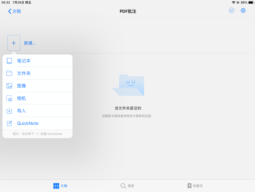
\includegraphics[width=0.45\textwidth]{05goodnotes/04importmenu}};
      \node[anchor=south west, inner sep=0, right=0.1 of img1](img2) 
      {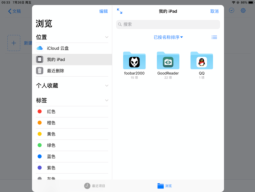
\includegraphics[width=0.45\textwidth]{05goodnotes/05importmyipad}};

      \begin{scope}[x={(img2.south east)},y={(img1.north west)}]
        % 绘制坐标辅助网络
        % \draw[very thin, draw=\finegridcolor, step=0.02] (0,0) grid (1,1);
        % \draw[thin, draw=\maingridcolor, xstep=0.1, ystep=0.1] (0,0) grid (1,1);
        % \foreach \x in {0,1,...,9} {
        %   \node [anchor=north] at (\x/10,0) {\tiny 0.\x};
        % }
        % \node [anchor=north] at (1,0) {\tiny 1};

        % \foreach \y in {0,1,...,9} {
        %   \node [anchor=east] at (0,\y/10) {\tiny 0.\y};
        % }
        % \node [anchor=east] at (0,1) {\tiny 1};
        
        % 利用fit库绘制命名矩形
        \node[fit={(0.23,0.92) (0.268, 0.96)}, inner sep=0pt, draw=blue, thick] (pdffold) {};        
        \node[fit={(0.008,0.731) (0.073, 0.825)}, inner sep=0pt, draw=red, thick] (new) {};
        \node[fit={(0.008,0.4) (0.055, 0.445)}, inner sep=0pt, draw=red, thick] (import) {};
        \node[fit={(0.57,0.67) (0.66, 0.71)}, inner sep=0pt, draw=red, thick] (ipad) {};
        %\node[fit={(0.69,0.92) (0.78, 0.96)}, inner sep=0pt, draw=blue, thick] (icloudroot) {};
        \node[fit={(0.81,0.92) (0.85, 0.96)}, inner sep=0pt, draw=blue, thick] (ipadpdf) {};
        \node[fit={(0.805,0.58) (0.92, 0.74)}, inner sep=0pt, draw=red, thick] (pdfname) {};
        % 绘制箭头连线表示操作顺序
        \draw[-{Stealth[scale=0.8]}, blue, thick] (pdffold.west) to [out=180, in=90] (new.north);
        \draw[-{Stealth[scale=0.8]}, red, thick] (new.east) to [out=0,
        in=180]node[midway,circle,fill=black,inner sep=0pt,minimum
        size=3pt,text=white] {\scriptsize \sffamily 1} (import.west);
        
        \draw[-{Stealth[scale=0.8]}, red, thick] (import.east) to
        [out=0, in=180]node[midway,circle,fill=black,inner
        sep=0pt,minimum size=3pt,text=white] {\scriptsize \sffamily 2}
        (ipad.west);
        
        \draw[-{Stealth[scale=0.8]}, red, thick] (ipad.east) to
        [out=0, in=180]node[midway,circle,fill=black,inner
        sep=0pt,minimum size=3pt,text=white] {\scriptsize \sffamily 3}
        (pdfname.west);
        
        \draw[-{Stealth[scale=0.8]}, blue, thick] (ipadpdf.south) to [out=-90, in=90] (pdfname.north);
      \end{scope}
    \end{tikzpicture}
  \end{center}
\end{frame}


\begin{frame}{iOS平板}{Goodnotes}
  \begin{itemize}\itemsep=3pt
  \item 打开PDF文件
    \begin{itemize}
    \item 进入\enquote{PDF批注}文件夹
    \item 从邮件\enquote{附件}打开
    \end{itemize}
  \end{itemize}
  \begin{center}
    % node [midway, sloped, above] {}
    \begin{annotationimage}{width=0.5\textwidth}{05goodnotes/06openfrommail}        
      % 利用fit库绘制命名矩形             
      \node[fit={(0.015,0.65) (0.31, 0.77)}, inner sep=0pt, draw=red, thick] (mailitem) {};
      \node[fit={(0.328,0.365) (0.5, 0.55)}, inner sep=0pt, draw=red, thick] (attachfile) {};
      \node[fit={(0.795,0.37) (0.89, 0.53)}, inner sep=0pt, draw=blue, thick] (goodnotessel) {};
      % % 绘制箭头连线表示操作顺序
      \draw[-{Stealth[scale=0.8]}, red, thick] (mailitem.south) to
      [out=-90, in=180]node [midway, sloped, below] {\small 打开邮件}
      (attachfile.west);
      
      \draw[-{Stealth[scale=0.8]}, blue, thick] (attachfile.north) to
      [out=90, in=90]node [midway, sloped, above] {\small 长按并选择
        \enquote{GoodNotes}}  (goodnotessel.north);      
    \end{annotationimage}
  \end{center}
\end{frame}

\begin{frame}{iOS平板}{Goodnotes}
  \begin{itemize}\itemsep=3pt
  \item 打开PDF文件
    \begin{itemize}
    \item 进入\enquote{PDF批注}文件夹
    \item 从\alert{Safari}\enquote{浏览器}打开
    \end{itemize}
  \end{itemize}
  \begin{center}
    % node [midway, sloped, above] {}
    \begin{annotationimage}{width=0.5\textwidth}{05goodnotes/06openfromsafra}
    %\begin{annotationimage}[grid]{width=0.5\textwidth}{05goodnotes/06openfromsafra}          
      % 利用fit库绘制命名矩形             
      \node[fit={(0.844,0.92) (0.88, 0.97)}, inner sep=0pt, draw=red, thick] (openwithothers) {};
      \node[fit={(0.885,0.53) (0.98, 0.69)}, inner sep=0pt, draw=blue, thick] (goodnotessel) {};
      % % 绘制箭头连线表示操作顺序      
      \draw[-{Stealth[scale=0.8]}, blue, thick] (openwithothers.south) to
      [out=-90, in=90]node [midway, sloped, above] {\tiny 点按并选择}  (goodnotessel.north);      
    \end{annotationimage}
  \end{center}
\end{frame}

\begin{frame}{iOS平板}{Goodnotes}
  \begin{itemize}\itemsep=3pt
  \item 打开PDF文件
    \begin{itemize}
    \item 进入\enquote{PDF批注}文件夹
    \item 从\alert{QQ}\enquote{传输文件}打开
    \end{itemize}
  \end{itemize}
  \begin{center}
    \begin{tikzpicture}
      \node[anchor=south west, inner sep=0](img1) at (0,0)
      {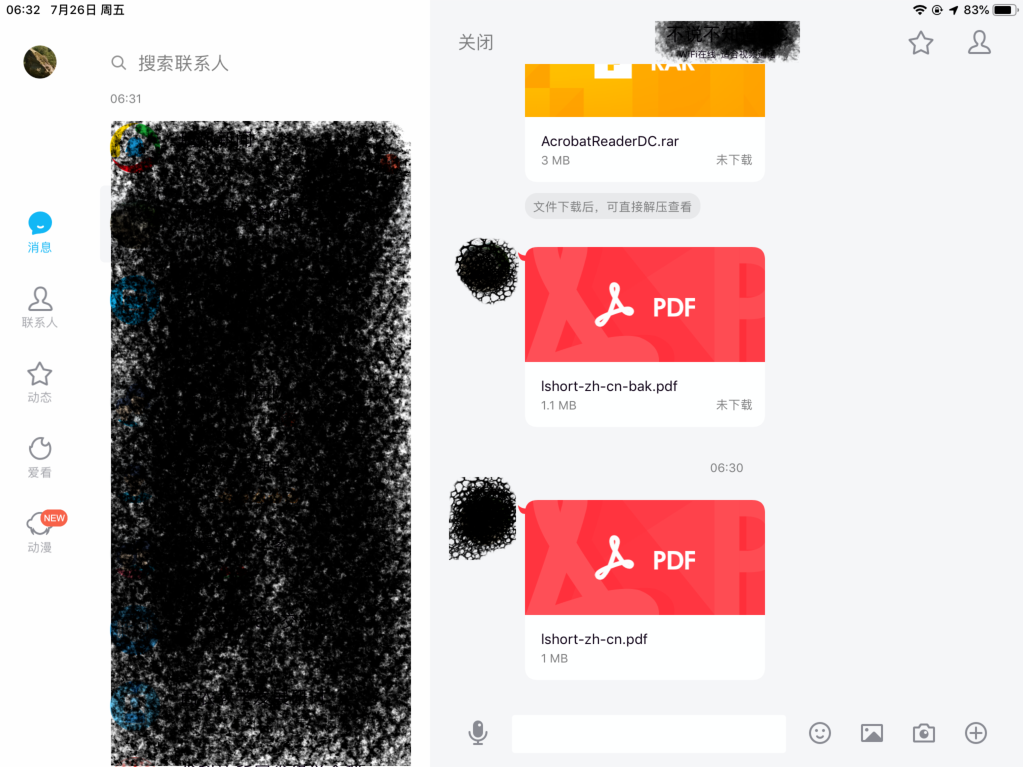
\includegraphics[width=0.34\textwidth]{05goodnotes/07qqfile}};
      \node[anchor=south west, inner sep=0, right=0.1 of img1](img2) 
      {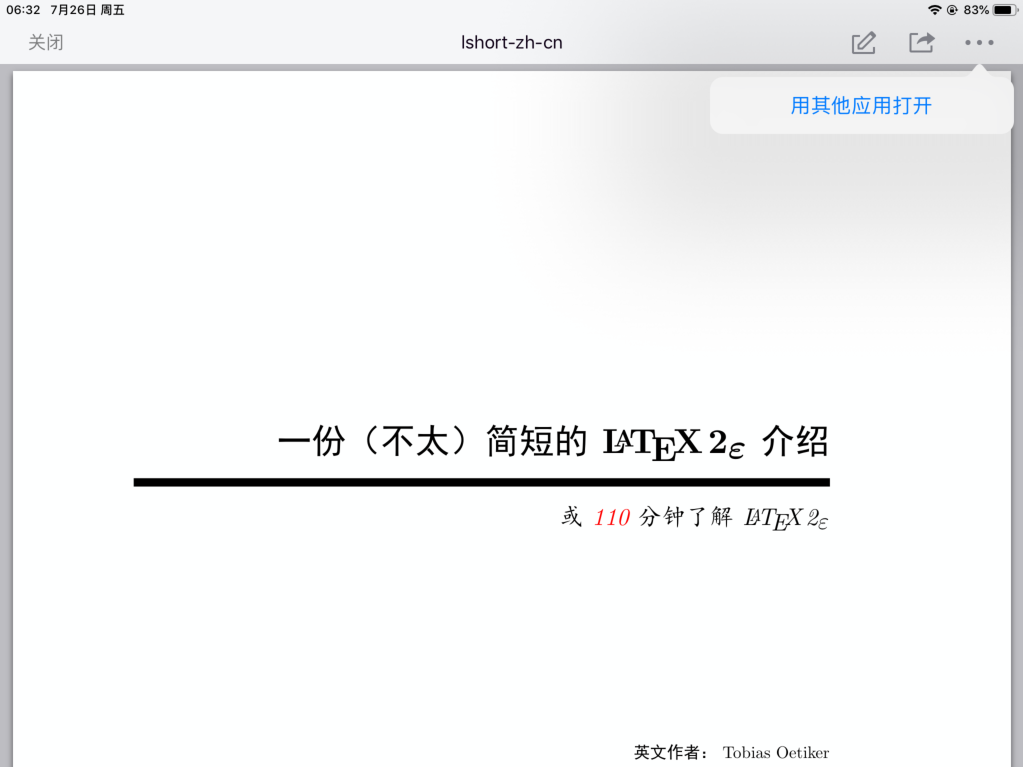
\includegraphics[width=0.34\textwidth]{05goodnotes/07openinqq}};
      \node[anchor=south west, inner sep=0, right=0.1 of img2](img3) 
      {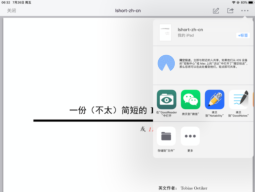
\includegraphics[width=0.34\textwidth]{05goodnotes/07qqopenwith}};

      \begin{scope}[x={(img3.south east)},y={(img1.north west)}]
        % 绘制坐标辅助网络
        % \draw[very thin, draw=\finegridcolor, step=0.02] (0,0) grid (1,1);
        % \draw[thin, draw=\maingridcolor, xstep=0.1, ystep=0.1] (0,0) grid (1,1);
        % \foreach \x in {0,1,...,9} {
        %   \node [anchor=north] at (\x/10,0) {\tiny 0.\x};
        % }
        % \node [anchor=north] at (1,0) {\tiny 1};

        % \foreach \y in {0,1,...,9} {
        %   \node [anchor=east] at (0,\y/10) {\tiny 0.\y};
        % }
        % \node [anchor=east] at (0,1) {\tiny 1};
        
        % 利用fit库绘制命名矩形
        \node[fit={(0.14,0.11) (0.27, 0.41)}, inner sep=0pt, draw=red, thick] (qqfile) {};        
        \node[fit={(0.64,0.925) (0.66, 0.958)}, inner sep=0pt, draw=red, thick] (qqfileopen) {};
        \node[fit={(0.56,0.81) (0.662, 0.905)}, inner sep=0pt,
        draw=red, thick] (qqopenwith) {};
        \node[fit={(0.96,0.38) (0.995, 0.537)}, inner sep=0pt, draw=red, thick] (goodnotessel) {};
        
        % 绘制箭头连线表示操作顺序
        \draw[-{Stealth[scale=0.8]}, red, thick] (qqfile.east) to [out=0,
        in=180]node[midway,circle,fill=black,inner sep=0pt,minimum
        size=3pt,text=white] {\scriptsize \sffamily 1} (qqfileopen.west);
        
        \draw[-{Stealth[scale=0.8]}, red, thick] (qqfileopen.east) to
        [out=0, in=0]node[midway,circle,fill=black,inner
        sep=0pt,minimum size=3pt,text=white] {\scriptsize \sffamily 2}
        (qqopenwith.east);
        
        \draw[-{Stealth[scale=0.8]}, red, thick] (qqopenwith.east) to
        [out=0, in=180]node[midway,circle,fill=black,inner
        sep=0pt,minimum size=3pt,text=white] {\scriptsize \sffamily 3}
        (goodnotessel.west);
      \end{scope}
    \end{tikzpicture}
  \end{center}
\end{frame}

\begin{frame}{iOS平板}{Goodnotes}
  \begin{itemize}\itemsep=3pt
  \item 打开PDF文件
    \begin{itemize}
    \item 进入\enquote{PDF批注}文件夹
    \item 从\alert{微信}\enquote{传输文件}打开
    \end{itemize}
  \end{itemize}
  \vspace{-1.5ex}
  \begin{center}
    \begin{tikzpicture}
      \node[anchor=south west, inner sep=0](img1) at (0,0)
      {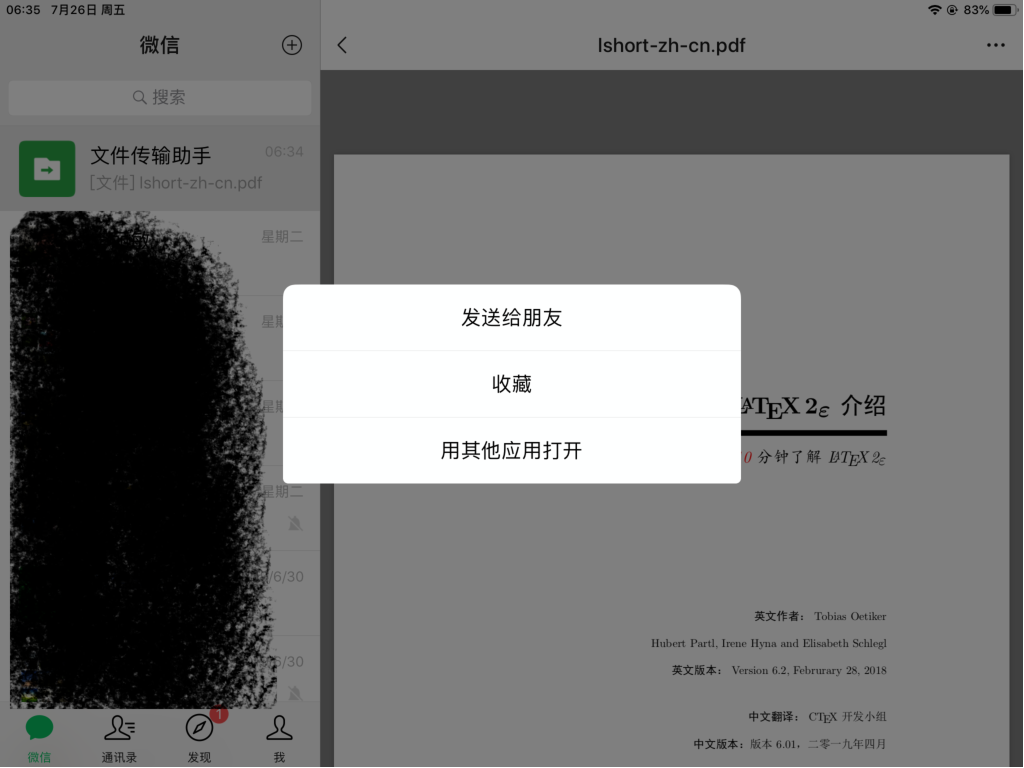
\includegraphics[width=0.48\textwidth]{05goodnotes/08wechatopentwithmenu}};
      \node[anchor=south west, inner sep=0, right=0.1 of img1](img2) 
      {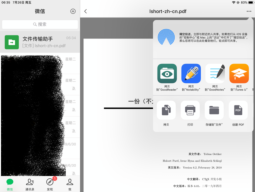
\includegraphics[width=0.48\textwidth]{05goodnotes/08wechatopenwithgoodnotes}};

      \begin{scope}[x={(img2.south east)},y={(img1.north west)}]
        % 绘制坐标辅助网络
        % \draw[very thin, draw=\finegridcolor, step=0.02] (0,0) grid (1,1);
        % \draw[thin, draw=\maingridcolor, xstep=0.1, ystep=0.1] (0,0) grid (1,1);
        % \foreach \x in {0,1,...,9} {
        %   \node [anchor=north] at (\x/10,0) {\tiny 0.\x};
        % }
        % \node [anchor=north] at (1,0) {\tiny 1};

        % \foreach \y in {0,1,...,9} {
        %   \node [anchor=east] at (0,\y/10) {\tiny 0.\y};
        % }
        % \node [anchor=east] at (0,1) {\tiny 1};
        
        % 利用fit库绘制命名矩形
        \node[fit={(0.47,0.93) (0.495, 0.955)}, inner sep=0pt, draw=blue, thick] (others) {};        
        \node[fit={(0.135,0.364) (0.36, 0.636)}, inner sep=0pt, draw=blue, thick] (openmenu) {};
        \node[fit={(0.21,0.395) (0.285, 0.432)}, inner sep=0pt,draw=red, thick] (openwith) {};
        \node[fit={(0.898,0.52) (0.942, 0.672)}, inner sep=0pt, draw=red, thick] (goodnotessel) {};
        
        % 绘制箭头连线表示操作顺序
        \draw[-{Stealth[scale=0.8]}, blue, thick] (others.west) to [out=-135,
        in=90]node[midway,circle,fill=black,inner sep=0pt,minimum
        size=3pt,text=white] {\scriptsize \sffamily 1} (openmenu.north);
        
        \draw[-{Stealth[scale=0.8]}, red, thick] (openwith.east) to
        [out=0, in=135]node[midway,circle,fill=black,inner
        sep=0pt,minimum size=3pt,text=white] {\scriptsize \sffamily 2}
        (goodnotessel.north);
        
        % \draw[-{Stealth[scale=0.8]}, red, thick] (qqopenwith.east) to
        % [out=0, in=180]node[midway,circle,fill=black,inner
        % sep=0pt,minimum size=3pt,white] {\scriptsize \sffamily 3}
        % (goodnotessel.west);
      \end{scope}
    \end{tikzpicture}
  \end{center}
\end{frame}

\begin{frame}{iOS平板}{Goodnotes}
  \begin{itemize}\itemsep=3pt
  \item 操作PDF文件
    \begin{itemize}
    \item 进入\enquote{PDF批注}文件夹
    \item 选中后进行操作
    \end{itemize}
  \end{itemize}
  \begin{center}
    % node [midway, sloped, above] {}
    \begin{annotationimage}{width=0.5\textwidth}{05goodnotes/09importedpdffile}
    %\begin{annotationimage}[grid]{width=0.5\textwidth}{05goodnotes/09importedpdffile}          
      % 利用fit库绘制命名矩形             
      \node[fit={(0.458,0.922) (0.54, 0.96)}, inner sep=0pt, draw=blue, thick] (pdffold) {};
      \node[fit={(0.028,0.608) (0.20, 0.71)}, inner sep=0pt, draw=red, thick] (pdfname) {};
      \node[fit={(0.59,0.44) (0.885, 0.887)}, inner sep=0pt, draw=red, thick] (pdfop) {};
      % % 绘制箭头连线表示操作顺序      
      % \draw[-{Stealth[scale=0.8]}, blue, thick] (openwithothers.south) to
      % [out=-90, in=90]node [midway, sloped, above] {\tiny 点按并选择}  (goodnotessel.north); 
      
    \end{annotationimage}
  \end{center}
\end{frame}

\begin{frame}{iOS平板}{Goodnotes}
  \begin{itemize}\itemsep=3pt
  \item 批注PDF文件
    \begin{itemize}
    \item 点击选中的PDF文件
    \item 在批注工具栏中\alert{选择合适工具}进行批注
    \end{itemize}
  \end{itemize}
  \begin{center}
    \begin{annotationimage}{width=0.5\textwidth}{05goodnotes/10toolbar}
    %\begin{annotationimage}[grid]{width=0.5\textwidth}{05goodnotes/10toolbar}          
      % 利用fit库绘制命名矩形             
      \node[fit={(0.13,0.86) (0.87, 0.91)}, inner sep=0pt, draw=red, thick] (pdffold) {};
      \draw[annotation right = {批注工具栏 at 0.887}] to (0.849,0.887);
    \end{annotationimage}
  \end{center}
\end{frame}

\begin{frame}{iOS平板}{Goodnotes}
  \begin{itemize}\itemsep=3pt
  \item 批注PDF文件
    \begin{itemize}
    \item 利用\alert{放大镜}工具实现细节批注
    \end{itemize}
  \end{itemize}
  \begin{center}
    \begin{annotationimage}{width=0.5\textwidth}{05goodnotes/11magnifier}
    %\begin{annotationimage}[grid]{width=0.55\textwidth}{05goodnotes/11magnifier}          
      % 利用fit库绘制命名矩形             
      \node[fit={(0.74,0.458) (0.97, 0.528)}, inner sep=0pt, draw=red, thick] (roi) {};
      \node[fit={(0.00,0.00) (1.00, 0.347)}, inner sep=0pt, draw=blue, thick] (magifier) {};
      % % 绘制箭头连线表示操作顺序      
      \draw[-{Stealth[scale=0.8]}, blue, thick] (roi.east) to
      [out=0, in=0]node [midway, sloped, above] {\tiny 区域放大}  (magifier.east); 
    \end{annotationimage}
  \end{center}
\end{frame}


\begin{frame}{iOS平板}{Goodnotes}
  \begin{itemize}\itemsep=3pt
  \item \enquote{批注}工具栏
    \begin{itemize}
    \item 工具类型
    \item 工具属性
    \end{itemize}
  \end{itemize}
  \begin{center}
    \begin{annotationimage}{width=0.8\textwidth}{05goodnotes/10toolbaricons}
    %\begin{annotationimage}[grid]{width=0.8\textwidth}{05goodnotes/10toolbaricons}
      % 绘制外观设置按钮分组示意下划线
      \draw[thick,blue] (0.62,0.10) -- (0.87,0.10);
      % 添加各图标标注
      \foreach \ann/\xpos in
      {
        {放\\大\\镜\\工\\具}/0.15, {钢\\笔\\工\\具}/0.20,
        {橡\\皮\\擦\\工\\具}/0.26, {萤\\光\\笔\\工\\具}/0.314,
        {绘\\图\\工\\具}/0.368, {索\\套\\选\\择\\工\\具}/0.424,
        {插\\图\\工\\具}/0.475, {拍\\照\\工\\具}/0.53,
        {文\\字\\输\\入\\工\\具}/0.585, {属\\性\\设\\置}/0.75
      }
      {
        \draw[annotation below = {{\ann} at \xpos}] to (\xpos,0.185);
      }
    \end{annotationimage}
  \end{center}
\end{frame}

\begin{frame}{iOS平板}{Goodnotes}
  \begin{itemize}\itemsep=3pt
  \item \enquote{批注}工具属性设置
    \begin{itemize}
    \item 点按工具图标\alert{两次}进行工具设置
    \item 在属性设计区设置颜色、宽度等属性
    \end{itemize}
  \end{itemize}
  \begin{center}
    \begin{tikzpicture}[font=\small]
      \node[anchor=south west, inner sep=0](img1) at (0,0)
      {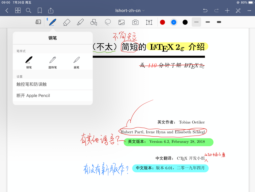
\includegraphics[width=0.35\textwidth]{05goodnotes/12pen}};
      
      \node[anchor=south west, inner sep=0, right=0.1 of img1](img2) 
      {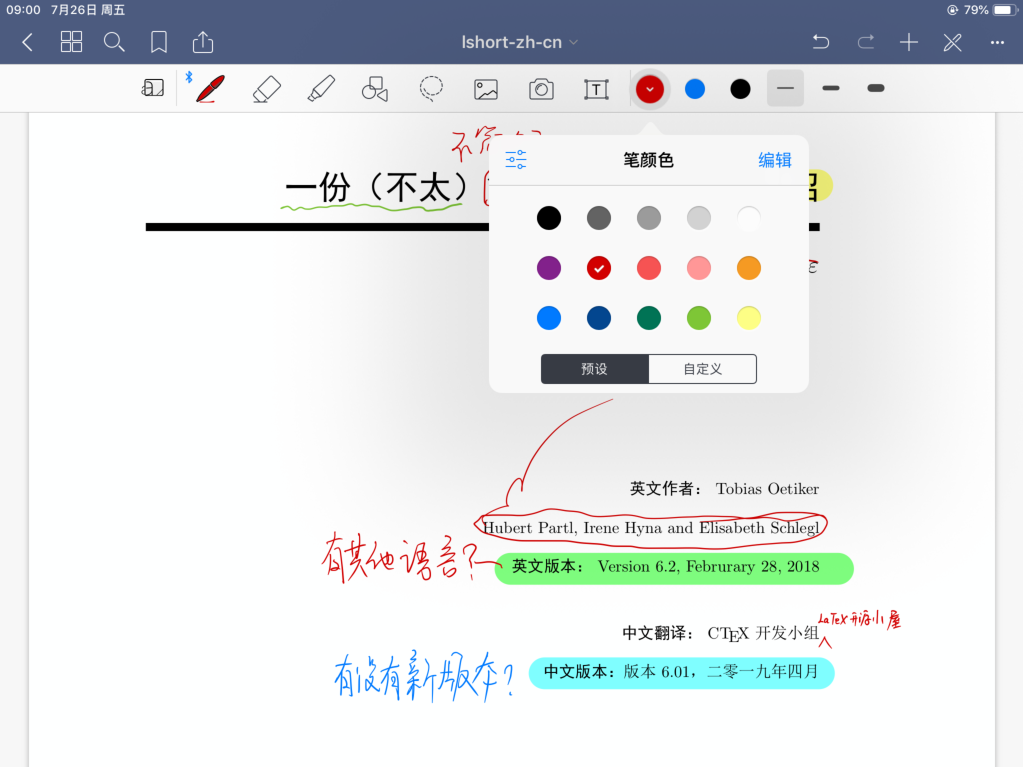
\includegraphics[width=0.35\textwidth]{05goodnotes/12pencol}};

      \node[anchor=south west, inner sep=0, right=0.1 of img2](img3) 
      {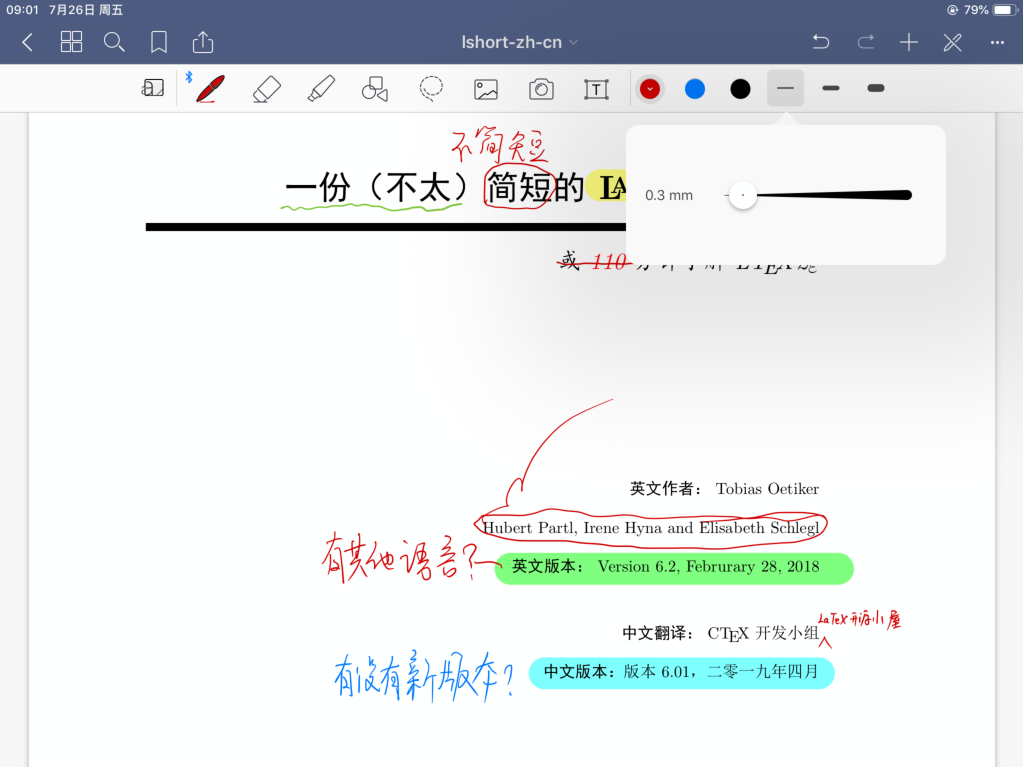
\includegraphics[width=0.35\textwidth]{05goodnotes/12penwidth}};

      \node[anchor=south west, inner sep=2pt, above=0.5 of img2,draw,blue,thick](txt)
      {钢笔设置};

      \begin{scope}[x={(img3.south east)},y={(img1.north west)}]
        % %绘制坐标辅助网络
        % \draw[very thin, draw=\finegridcolor, step=0.02] (0,0) grid (1,1);
        % \draw[thin, draw=\maingridcolor, xstep=0.1, ystep=0.1] (0,0) grid (1,1);
        % \foreach \x in {0,1,...,9} {
        %   \node [anchor=north] at (\x/10,0) {\tiny 0.\x};
        % }
        % \node [anchor=north] at (1,0) {\tiny 1};

        % \foreach \y in {0,1,...,9} {
        %   \node [anchor=east] at (0,\y/10) {\tiny 0.\y};
        % }
        % \node [anchor=east] at (0,1) {\tiny 1};
        
        % 利用fit库绘制命名矩形
        \node[fit={(0.015,0.45) (0.12, 0.84)}, inner sep=0pt, draw=red, thick] (pen) {}; 
        \node[fit={(0.492,0.493) (0.595, 0.827)}, inner sep=0pt, draw=red, thick] (pencol) {};
        \node[fit={(0.872,0.65) (0.976, 0.84)}, inner sep=0pt, draw=red, thick] (penwidth) {}; 
        % % 绘制箭头连线表示操作顺序
        \draw[-{Stealth[scale=0.8]}, red, thick] (txt.west) to [out=180,
        in=0]node[midway, sloped, above] {笔类型} (pen.east);

        \draw[-{Stealth[scale=0.8]}, red, thick] (txt.south) to [out=-135,
        in=180]node[midway, sloped, above] {笔颜色} (pencol.west);

        \draw[-{Stealth[scale=0.8]}, red, thick] (txt.east) to [out=0,
        in=180]node[midway, sloped, above] {笔宽度} (penwidth.west);
      \end{scope}
    \end{tikzpicture}
  \end{center}
\end{frame}

\begin{frame}{iOS平板}{Goodnotes}
  \begin{itemize}\itemsep=3pt
  \item \enquote{批注}工具属性设置
    \begin{itemize}
    \item 点按工具图标\alert{两次}进行工具设置
    \item 在属性设计区设置颜色、宽度等属性
    \end{itemize}
  \end{itemize}
  \vspace{-3ex}
  \begin{center}
    \begin{tikzpicture}[font=\small]
      \node[anchor=south west, inner sep=0](img1) at (0,0)
      {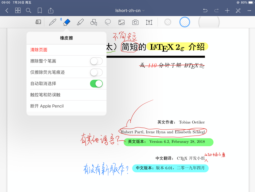
\includegraphics[width=0.45\textwidth]{05goodnotes/13erase}};

      \node[anchor=south west, inner sep=2pt, above=0.2 of img1,draw,blue,thick](txt)
      {橡皮擦设置};

      \begin{scope}[x={(img1.south east)},y={(img1.north west)}]
        % %绘制坐标辅助网络
        % \draw[very thin, draw=\finegridcolor, step=0.02] (0,0) grid (1,1);
        % \draw[thin, draw=\maingridcolor, xstep=0.1, ystep=0.1] (0,0) grid (1,1);
        % \foreach \x in {0,1,...,9} {
        %   \node [anchor=north] at (\x/10,0) {\tiny 0.\x};
        % }
        % \node [anchor=north] at (1,0) {\tiny 1};

        % \foreach \y in {0,1,...,9} {
        %   \node [anchor=east] at (0,\y/10) {\tiny 0.\y};
        % }
        % \node [anchor=east] at (0,1) {\tiny 1};
        
        % 利用fit库绘制命名矩形
        \node[fit={(0.1,0.4) (0.42, 0.84)}, inner sep=0pt, draw=red, thick] (eraser) {}; 
        \node[fit={(0.627,0.852) (0.87, 0.917)}, inner sep=0pt, draw=red, thick] (erasersize) {};
        % % 绘制箭头连线表示操作顺序
        \draw[-{Stealth[scale=0.8]}, red, thick] (txt.west) to [out=180,
        in=180]node[midway, sloped, above] {橡皮擦属性} (eraser.west);

        \draw[-{Stealth[scale=0.8]}, red, thick] (txt.east) to [out=0,
        in=90]node[midway, sloped, above] {橡皮檫大小} (erasersize.north);
      \end{scope}
    \end{tikzpicture}
  \end{center}
\end{frame}

\begin{frame}{iOS平板}{Goodnotes}
  \begin{itemize}\itemsep=3pt
  \item \enquote{批注}工具属性设置
    \begin{itemize}
    \item 点按工具图标\alert{两次}进行工具设置
    \item 在属性设计区设置颜色、宽度等属性
    \end{itemize}
  \end{itemize}
  \begin{center}
    \begin{tikzpicture}[font=\small]
      \node[anchor=south west, inner sep=0](img1) at (0,0)
      {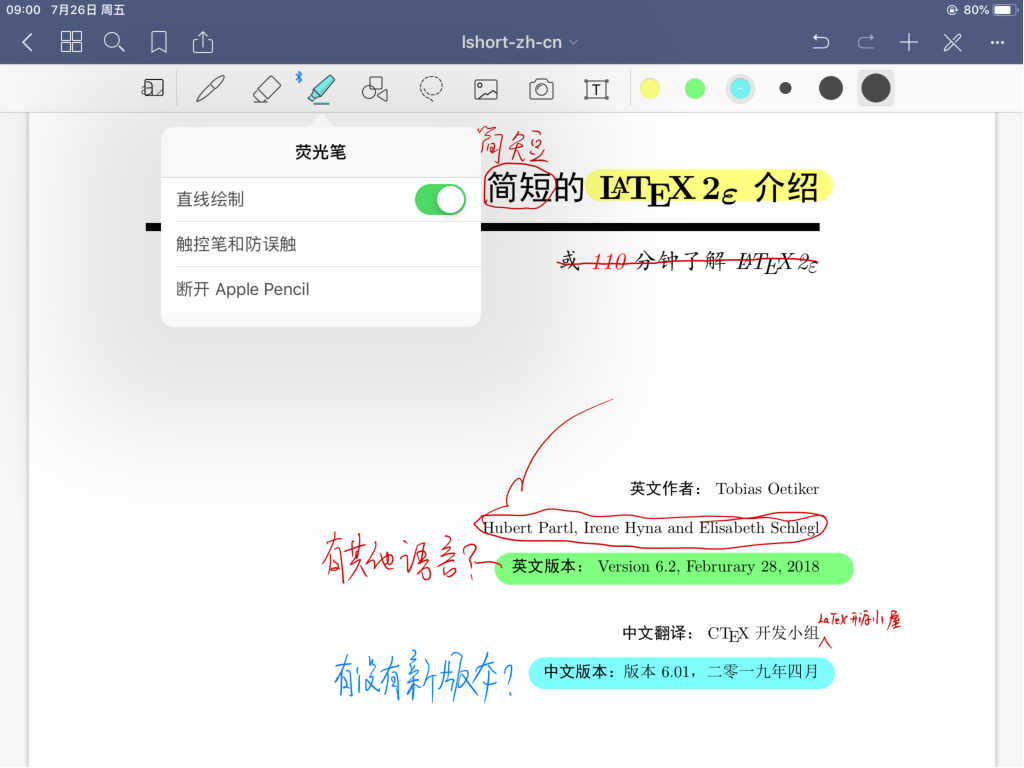
\includegraphics[width=0.35\textwidth]{05goodnotes/14highlightpen}};
      
      \node[anchor=south west, inner sep=0, right=0.1 of img1](img2) 
      {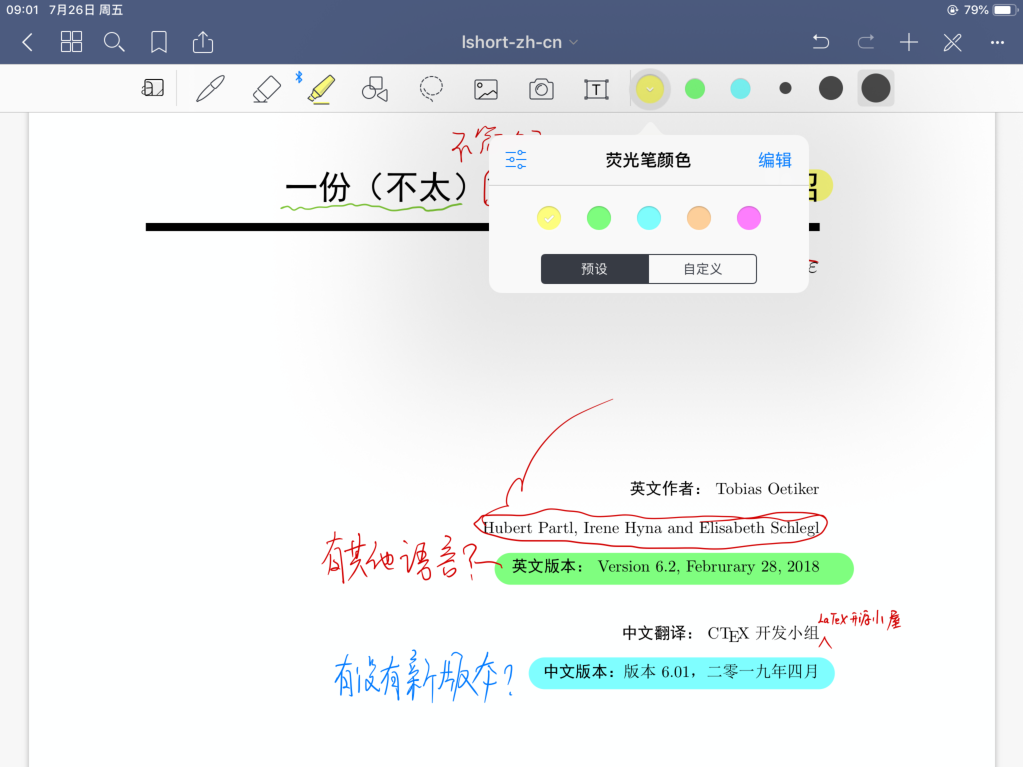
\includegraphics[width=0.35\textwidth]{05goodnotes/14highlightpencol}};

      \node[anchor=south west, inner sep=0, right=0.1 of img2](img3) 
      {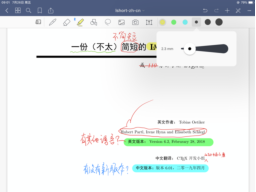
\includegraphics[width=0.35\textwidth]{05goodnotes/14highlightpenwidth}};

      \node[anchor=south west, inner sep=2pt, above=0.5 of img2,draw,blue,thick](txt)
      {萤光笔设置};

      \begin{scope}[x={(img3.south east)},y={(img1.north west)}]
        % %绘制坐标辅助网络
        % \draw[very thin, draw=\finegridcolor, step=0.02] (0,0) grid (1,1);
        % \draw[thin, draw=\maingridcolor, xstep=0.1, ystep=0.1] (0,0) grid (1,1);
        % \foreach \x in {0,1,...,9} {
        %   \node [anchor=north] at (\x/10,0) {\tiny 0.\x};
        % }
        % \node [anchor=north] at (1,0) {\tiny 1};

        % \foreach \y in {0,1,...,9} {
        %   \node [anchor=east] at (0,\y/10) {\tiny 0.\y};
        % }
        % \node [anchor=east] at (0,1) {\tiny 1};
        
        % 利用fit库绘制命名矩形
        \node[fit={(0.052,0.578) (0.154, 0.84)}, inner sep=0pt, draw=red, thick] (pen) {}; 
        \node[fit={(0.492,0.615) (0.595, 0.827)}, inner sep=0pt, draw=red, thick] (pencol) {};
        \node[fit={(0.872,0.65) (0.976, 0.84)}, inner sep=0pt, draw=red, thick] (penwidth) {}; 
        % % 绘制箭头连线表示操作顺序
        \draw[-{Stealth[scale=0.8]}, red, thick] (txt.west) to [out=180,
        in=0]node[midway, sloped, above] {萤光笔类型} (pen.east);

        \draw[-{Stealth[scale=0.8]}, red, thick] (txt.south) to [out=-135,
        in=180]node[midway, sloped, above] {萤光笔颜色} (pencol.west);

        \draw[-{Stealth[scale=0.8]}, red, thick] (txt.east) to [out=0,
        in=180]node[midway, sloped, above] {萤光笔宽度} (penwidth.west);
      \end{scope}
    \end{tikzpicture}
  \end{center}
\end{frame}

\begin{frame}{iOS平板}{Goodnotes}
  \begin{itemize}\itemsep=3pt
  \item \enquote{批注}工具属性设置
    \begin{itemize}
    \item 点按工具图标\alert{两次}进行工具设置
    \item 在属性设计区设置颜色、宽度等属性
    \end{itemize}
  \end{itemize}
  \begin{center}
    \begin{tikzpicture}[font=\small]
      \node[anchor=south west, inner sep=0](img1) at (0,0)
      {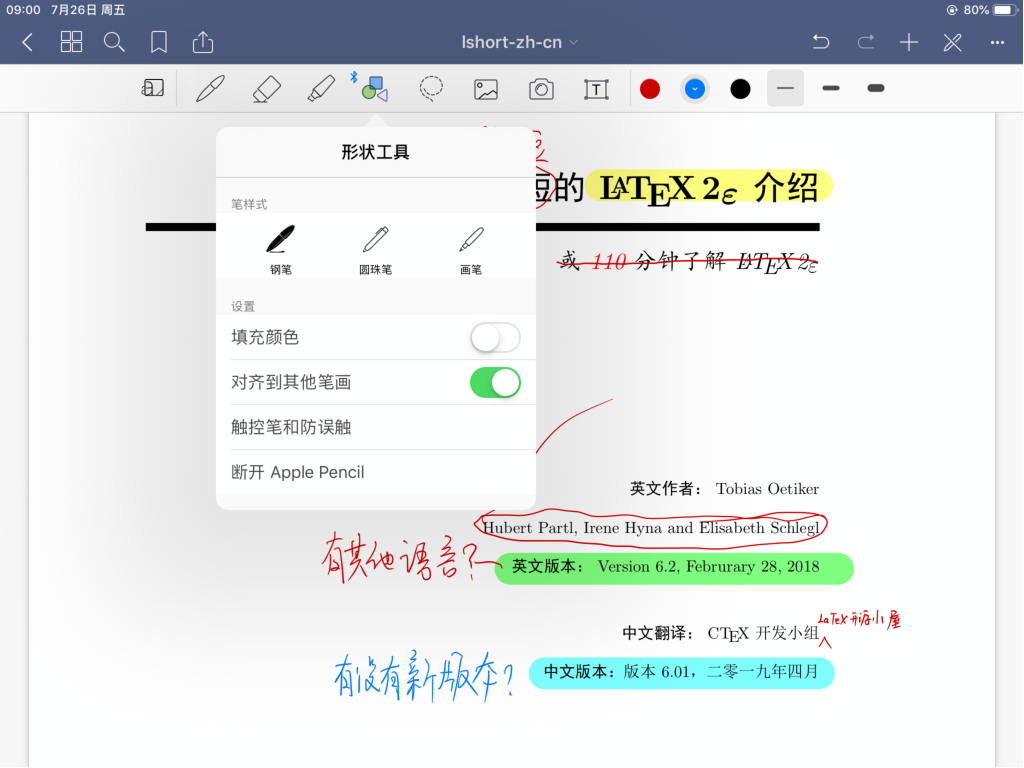
\includegraphics[width=0.35\textwidth]{05goodnotes/15drawtools}};
      
      \node[anchor=south west, inner sep=0, right=0.1 of img1](img2) 
      {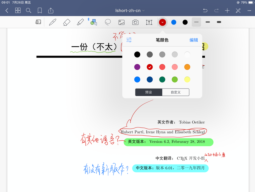
\includegraphics[width=0.35\textwidth]{05goodnotes/15drawtoolscol}};

      \node[anchor=south west, inner sep=0, right=0.1 of img2](img3) 
      {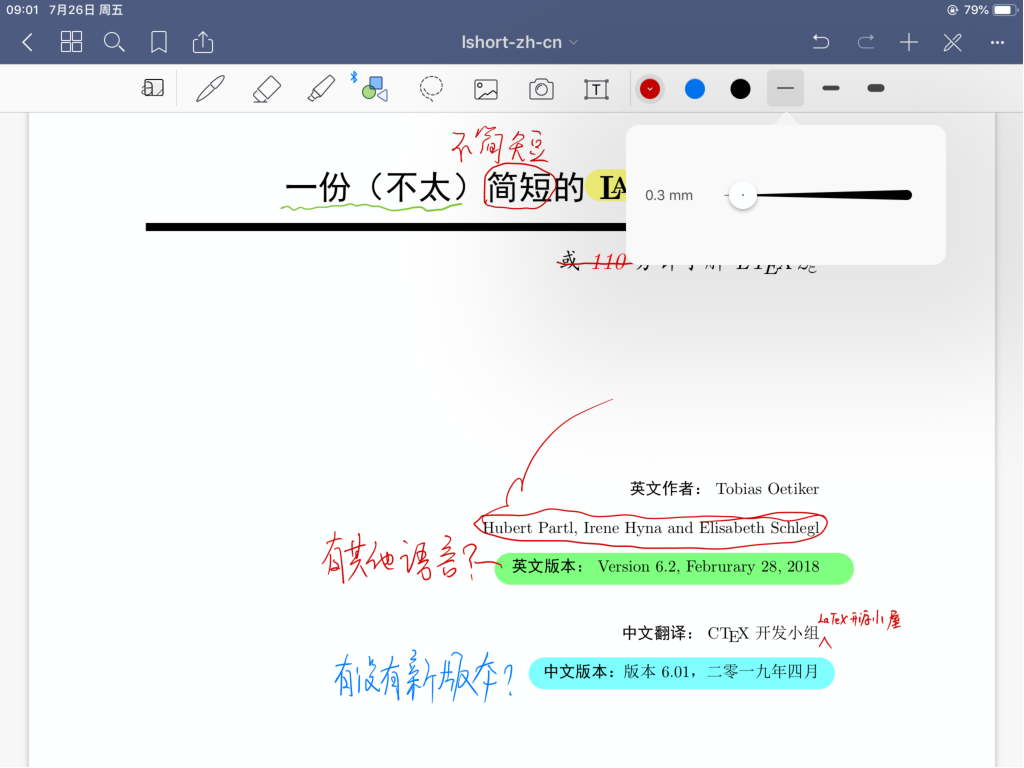
\includegraphics[width=0.35\textwidth]{05goodnotes/15drawtoolswidth}};

      \node[anchor=south west, inner sep=2pt, above=0.5 of img2,draw,blue,thick](txt)
      {形状工具设置};

      \begin{scope}[x={(img3.south east)},y={(img1.north west)}]
        % %绘制坐标辅助网络
        % \draw[very thin, draw=\finegridcolor, step=0.02] (0,0) grid (1,1);
        % \draw[thin, draw=\maingridcolor, xstep=0.1, ystep=0.1] (0,0) grid (1,1);
        % \foreach \x in {0,1,...,9} {
        %   \node [anchor=north] at (\x/10,0) {\tiny 0.\x};
        % }
        % \node [anchor=north] at (1,0) {\tiny 1};

        % \foreach \y in {0,1,...,9} {
        %   \node [anchor=east] at (0,\y/10) {\tiny 0.\y};
        % }
        % \node [anchor=east] at (0,1) {\tiny 1};
        
        % 利用fit库绘制命名矩形
        \node[fit={(0.069,0.338) (0.173, 0.84)}, inner sep=0pt, draw=red, thick] (draw) {}; 
        \node[fit={(0.492,0.48) (0.595, 0.827)}, inner sep=0pt, draw=red, thick] (drawcol) {};
        \node[fit={(0.872,0.65) (0.976, 0.84)}, inner sep=0pt, draw=red, thick] (drawwidth) {}; 
        % % 绘制箭头连线表示操作顺序
        \draw[-{Stealth[scale=0.8]}, red, thick] (txt.west) to [out=180,
        in=0]node[midway, sloped, above] {形状属性} (draw.east);

        \draw[-{Stealth[scale=0.8]}, red, thick] (txt.south) to [out=-135,
        in=180]node[midway, sloped, above] {形状颜色} (drawcol.west);

        \draw[-{Stealth[scale=0.8]}, red, thick] (txt.east) to [out=0,
        in=180]node[midway, sloped, above] {线条宽度} (drawwidth.west);
      \end{scope}
    \end{tikzpicture}
  \end{center}
\end{frame}

\begin{frame}{iOS平板}{Goodnotes}
  \begin{itemize}\itemsep=3pt
  \item \enquote{批注}工具属性设置
    \begin{itemize}
    \item 点按工具图标\alert{两次}进行工具设置
    \item 在属性设计区设置颜色、宽度等属性
    \end{itemize}
  \end{itemize}
  %\vspace{-2ex}
  \begin{center}
    \begin{tikzpicture}[font=\small]
      \node[anchor=south west, inner sep=0](img1) at (0,0)
      {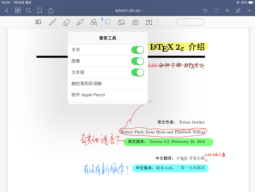
\includegraphics[width=0.45\textwidth]{05goodnotes/16seltool}};

      \node[anchor=south west, inner sep=2pt, above=0.2 of img1,draw,blue,thick](txt)
      {索套设置};

      \begin{scope}[x={(img1.south east)},y={(img1.north west)}]
        % %绘制坐标辅助网络
        % \draw[very thin, draw=\finegridcolor, step=0.02] (0,0) grid (1,1);
        % \draw[thin, draw=\maingridcolor, xstep=0.1, ystep=0.1] (0,0) grid (1,1);
        % \foreach \x in {0,1,...,9} {
        %   \node [anchor=north] at (\x/10,0) {\tiny 0.\x};
        % }
        % \node [anchor=north] at (1,0) {\tiny 1};

        % \foreach \y in {0,1,...,9} {
        %   \node [anchor=east] at (0,\y/10) {\tiny 0.\y};
        % }
        % \node [anchor=east] at (0,1) {\tiny 1};
        
        % 利用fit库绘制命名矩形
        \node[fit={(0.262,0.46) (0.579, 0.84)}, inner sep=0pt, draw=red, thick] (sel) {};
        % % 绘制箭头连线表示操作顺序
        \draw[-{Stealth[scale=0.8]}, red, thick] (txt.east) to [out=0,
        in=0]node[midway, sloped, above] {索套属性} (sel.east);
      \end{scope}
    \end{tikzpicture}
  \end{center}
\end{frame}

\begin{frame}{iOS平板}{Goodnotes}
  \begin{itemize}\itemsep=3pt
  \item \enquote{批注}工具属性设置
    \begin{itemize}
    \item 点按工具图标\alert{两次}进行工具设置
    \item 在属性设计区设置颜色、宽度等属性
    \end{itemize}
  \end{itemize}
  \vspace{-1ex}
  \begin{center}
    \begin{tikzpicture}[font=\small]
      \node[anchor=south west, inner sep=0](img1) at (0,0)
      {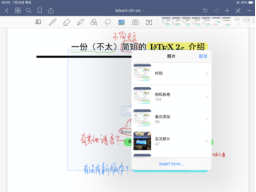
\includegraphics[width=0.45\textwidth]{05goodnotes/17image}};

      \node[anchor=south west, inner sep=2pt, above=0.2 of img1,draw,blue,thick](txt)
      {插入图像};

      \begin{scope}[x={(img1.south east)},y={(img1.north west)}]
        % %绘制坐标辅助网络
        % \draw[very thin, draw=\finegridcolor, step=0.02] (0,0) grid (1,1);
        % \draw[thin, draw=\maingridcolor, xstep=0.1, ystep=0.1] (0,0) grid (1,1);
        % \foreach \x in {0,1,...,9} {
        %   \node [anchor=north] at (\x/10,0) {\tiny 0.\x};
        % }
        % \node [anchor=north] at (1,0) {\tiny 1};

        % \foreach \y in {0,1,...,9} {
        %   \node [anchor=east] at (0,\y/10) {\tiny 0.\y};
        % }
        % \node [anchor=east] at (0,1) {\tiny 1};
        
        % 利用fit库绘制命名矩形
        \node[fit={(0.516,0.101) (0.823, 0.74)}, inner sep=0pt, draw=red, thick] (img) {};
        % % 绘制箭头连线表示操作顺序
        \draw[-{Stealth[scale=0.8]}, red, thick] (txt.east) to [out=0,
        in=90]node[midway, sloped, below] {选择图像来源} (img.north);
      \end{scope}
    \end{tikzpicture}
  \end{center}
\end{frame}

\begin{frame}{iOS平板}{Goodnotes}
  \begin{itemize}\itemsep=3pt
  \item \enquote{批注}工具属性设置
    \begin{itemize}
    \item 点按工具图标\alert{两次}进行工具设置
    \item 在属性设计区设置颜色、宽度等属性
    \end{itemize}
  \end{itemize}
  \vspace{-1ex}
  \begin{center}
    \begin{annotationimage}{width=0.45\textwidth}{05goodnotes/18camera}
      \node[anchor=south west, inner sep=2pt, above=0.04 of image,draw,blue,thick](txt)
      {插入相机图像};
      \draw[annotation right = {点击页面任意\\位置打开相机 at 0.4}] to (0.5,0.4);
    \end{annotationimage}
  \end{center}
\end{frame}

\begin{frame}{iOS平板}{Goodnotes}
  \begin{itemize}\itemsep=3pt
  \item \enquote{批注}工具属性设置
    \begin{itemize}
    \item 点按工具图标\alert{两次}进行工具设置
    \item 在属性设计区设置颜色、宽度等属性
    \end{itemize}
  \end{itemize}
  \begin{center}
    \begin{tikzpicture}[font=\small]
      \node[anchor=south west, inner sep=0](img1) at (0,0)
      {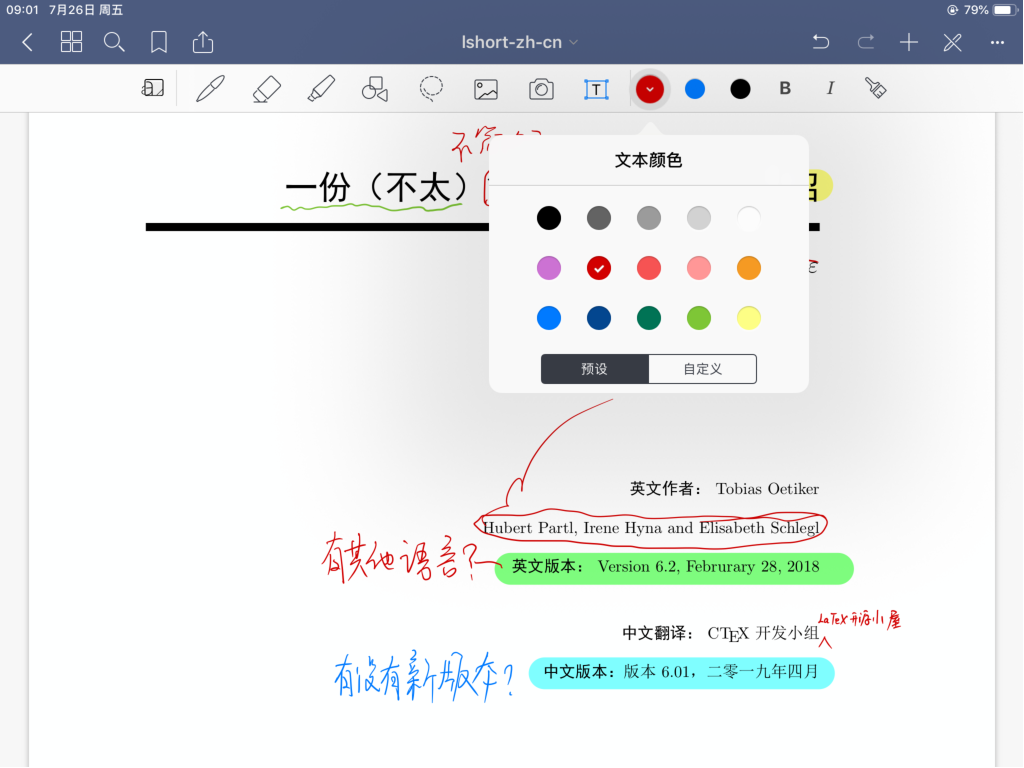
\includegraphics[width=0.45\textwidth]{05goodnotes/19textcol}};
      
      \node[anchor=south west, inner sep=0, right=0.1 of img1](img2) 
      {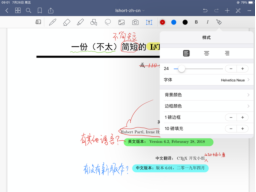
\includegraphics[width=0.45\textwidth]{05goodnotes/19textfmt}};

      \node[anchor=west, inner sep=2pt, above=0.2 of img2,xshift = -3.25cm,draw,blue,thick](txt)
      {文字属性设置};

      \begin{scope}[x={(img2.south east)},y={(img1.north west)}]
        % %绘制坐标辅助网络
        % \draw[very thin, draw=\finegridcolor, step=0.02] (0,0) grid (1,1);
        % \draw[thin, draw=\maingridcolor, xstep=0.1, ystep=0.1] (0,0) grid (1,1);
        % \foreach \x in {0,1,...,9} {
        %   \node [anchor=north] at (\x/10,0) {\tiny 0.\x};
        % }
        % \node [anchor=north] at (1,0) {\tiny 1};

        % \foreach \y in {0,1,...,9} {
        %   \node [anchor=east] at (0,\y/10) {\tiny 0.\y};
        % }
        % \node [anchor=east] at (0,1) {\tiny 1};
        
        % 利用fit库绘制命名矩形
        \node[fit={(0.238,0.49) (0.39, 0.82)}, inner sep=0pt, draw=red, thick] (txtcol) {}; 
        \node[fit={(0.815,0.28) (0.995, 0.84)}, inner sep=0pt, draw=red, thick] (txtfmt) {};
        % % 绘制箭头连线表示操作顺序
        \draw[-{Stealth[scale=0.8]}, red, thick] (txt.west) to [out=180,
        in=180]node[midway, sloped, above] {文字颜色} (txtcol.west);

        \draw[-{Stealth[scale=0.8]}, red, thick] (txt.east) to [out=0,
        in=180]node[midway, sloped, above] {文字样式} (txtfmt.west);
      \end{scope}
    \end{tikzpicture}
  \end{center}
\end{frame}

\begin{frame}{iOS平板}{Goodnotes}
  \begin{itemize}\itemsep=3pt
  \item \enquote{\alert{导出}}批注结果
    \begin{itemize}
    \item 点按\alert{导出}操作按钮
    \end{itemize}
  \end{itemize}
  \begin{center}
    \begin{tikzpicture}[font=\small]
      \node[anchor=south west, inner sep=0](img1) at (0,0)
      {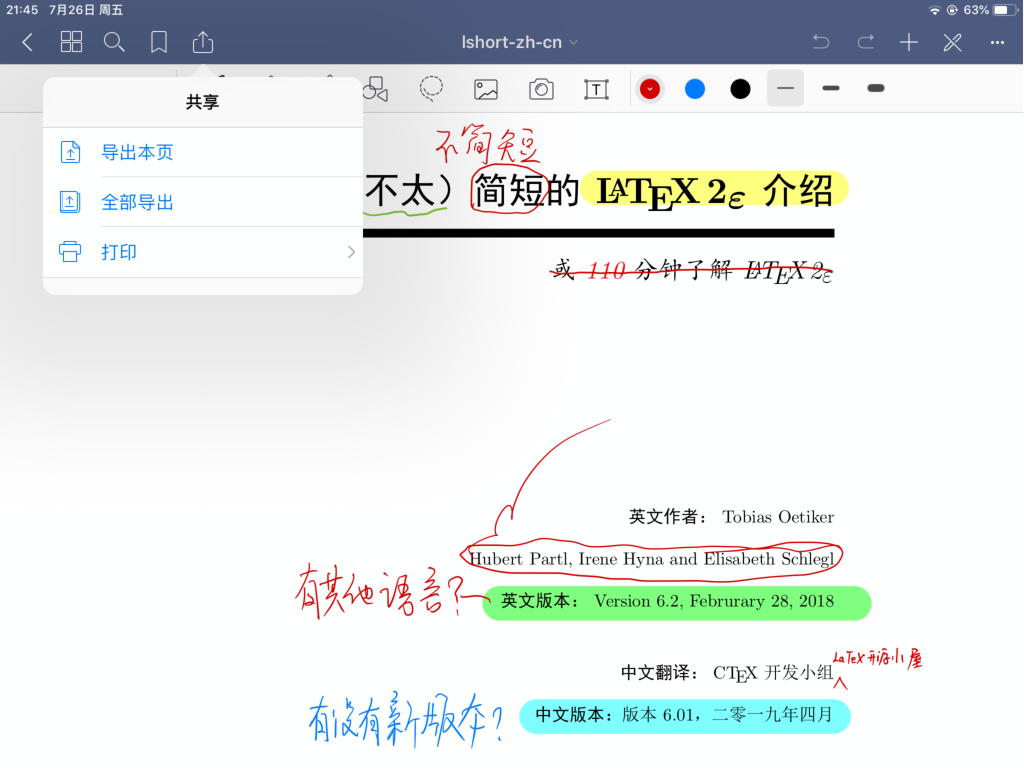
\includegraphics[width=0.55\textwidth]{05goodnotes/20exportmenu}};

      \begin{scope}[x={(img1.south east)},y={(img1.north west)}]
        % %绘制坐标辅助网络
        % \draw[very thin, draw=\finegridcolor, step=0.02] (0,0) grid (1,1);
        % \draw[thin, draw=\maingridcolor, xstep=0.1, ystep=0.1] (0,0) grid (1,1);
        % \foreach \x in {0,1,...,9} {
        %   \node [anchor=north] at (\x/10,0) {\tiny 0.\x};
        % }
        % \node [anchor=north] at (1,0) {\tiny 1};

        % \foreach \y in {0,1,...,9} {
        %   \node [anchor=east] at (0,\y/10) {\tiny 0.\y};
        % }
        % \node [anchor=east] at (0,1) {\tiny 1};
        
        % 利用fit库绘制命名矩形
        \node[fit={(0.18,0.92) (0.22, 0.97)}, inner sep=0pt, draw=blue, thick] (export) {}; 
        \node[fit={(0.039,0.618) (0.357, 0.9)}, inner sep=0pt, draw=red, thick] (menu) {};
        % % 绘制箭头连线表示操作顺序
        \draw[-{Stealth[scale=0.8]}, blue, thick] (export.east) to [out=0,
        in=0] (menu.east);
      \end{scope}
    \end{tikzpicture}
  \end{center}
\end{frame}

\begin{frame}{iOS平板}{Goodnotes}
  \begin{itemize}\itemsep=3pt
  \item \enquote{\alert{导出}}批注结果
    \begin{itemize}
    \item 选择导出\alert{格式}
    \end{itemize}
  \end{itemize}
  \begin{center}
    \begin{tikzpicture}[font=\small]
      \node[anchor=south west, inner sep=0](img1) at (0,0)
      {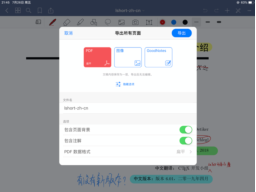
\includegraphics[width=0.55\textwidth]{05goodnotes/21exportsel}};

      \begin{scope}[x={(img1.south east)},y={(img1.north west)}]
        % %绘制坐标辅助网络
        % \draw[very thin, draw=\finegridcolor, step=0.02] (0,0) grid (1,1);
        % \draw[thin, draw=\maingridcolor, xstep=0.1, ystep=0.1] (0,0) grid (1,1);
        % \foreach \x in {0,1,...,9} {
        %   \node [anchor=north] at (\x/10,0) {\tiny 0.\x};
        % }
        % \node [anchor=north] at (1,0) {\tiny 1};

        % \foreach \y in {0,1,...,9} {
        %   \node [anchor=east] at (0,\y/10) {\tiny 0.\y};
        % }
        % \node [anchor=east] at (0,1) {\tiny 1};
        
        % 利用fit库绘制命名矩形
        \node[fit={(0.23,0.14) (0.768, 0.86)}, inner sep=0pt, draw=red, thick] (exportfmt) {};
      \end{scope}
    \end{tikzpicture}
  \end{center}
\end{frame}

\begin{frame}{iOS平板}{Goodnotes}
  \begin{itemize}\itemsep=3pt
  \item \enquote{\alert{导出}}批注结果
    \begin{itemize}
    \item 导出过程
    \end{itemize}
  \end{itemize}
  \begin{center}
    \begin{tikzpicture}[font=\small]
      \node[anchor=south west, inner sep=0](img1) at (0,0)
      {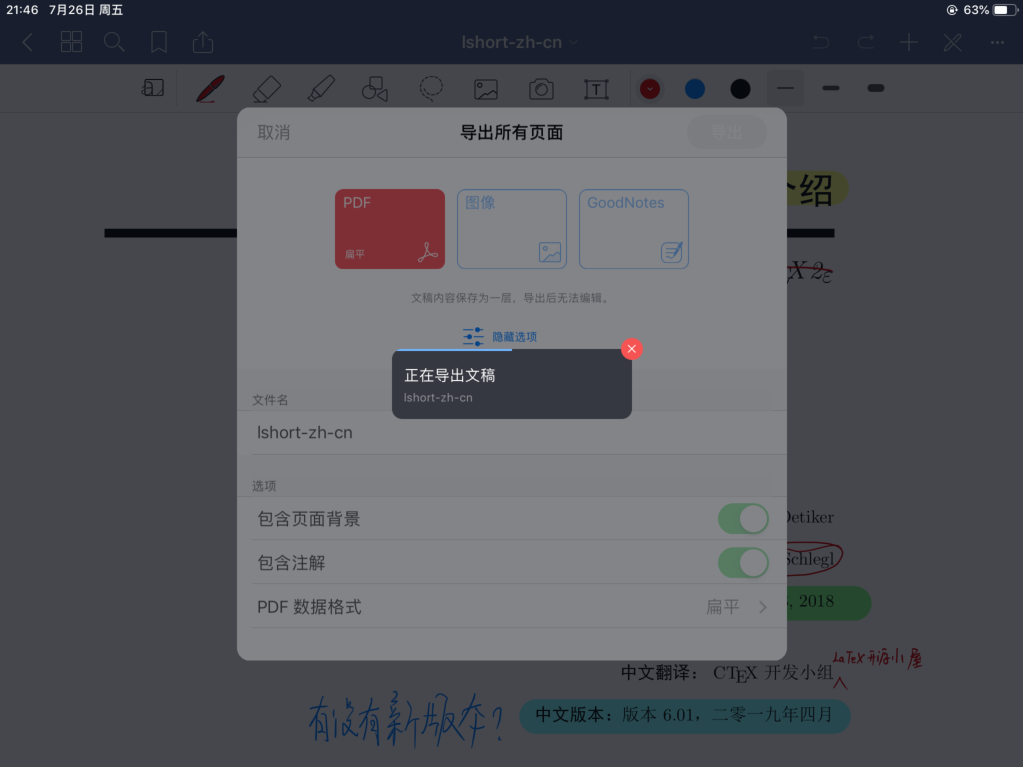
\includegraphics[width=0.55\textwidth]{05goodnotes/22exortprgbar}};

      \begin{scope}[x={(img1.south east)},y={(img1.north west)}]
        % %绘制坐标辅助网络
        % \draw[very thin, draw=\finegridcolor, step=0.02] (0,0) grid (1,1);
        % \draw[thin, draw=\maingridcolor, xstep=0.1, ystep=0.1] (0,0) grid (1,1);
        % \foreach \x in {0,1,...,9} {
        %   \node [anchor=north] at (\x/10,0) {\tiny 0.\x};
        % }
        % \node [anchor=north] at (1,0) {\tiny 1};

        % \foreach \y in {0,1,...,9} {
        %   \node [anchor=east] at (0,\y/10) {\tiny 0.\y};
        % }
        % \node [anchor=east] at (0,1) {\tiny 1};
        
        % 利用fit库绘制命名矩形
        \node[fit={(0.381,0.457) (0.630, 0.58)}, inner sep=0pt, draw=red, thick] (exportfmt) {};
      \end{scope}
    \end{tikzpicture}
  \end{center}
\end{frame}

\begin{frame}{iOS平板}{Goodnotes}
  \begin{columns}[T]
    \column{0.35\textwidth}
  \begin{itemize}\itemsep=8pt
  \item \enquote{\alert{导出}}批注结果
    \begin{itemize}\itemsep=8pt
    \item 选择发送方式
      \begin{itemize}\itemsep=10pt
      \item 邮件(\alert{强烈推荐})
      \item 微信
      \item QQ
      \item iTunes
      \item iClound
      \item \ldots
      \end{itemize}
    \end{itemize}
  \end{itemize}
    \column{0.55\textwidth}
  \begin{center}
    \begin{tikzpicture}[font=\small]
      \node[anchor=south west, inner sep=0](img1) at (0,0)
      {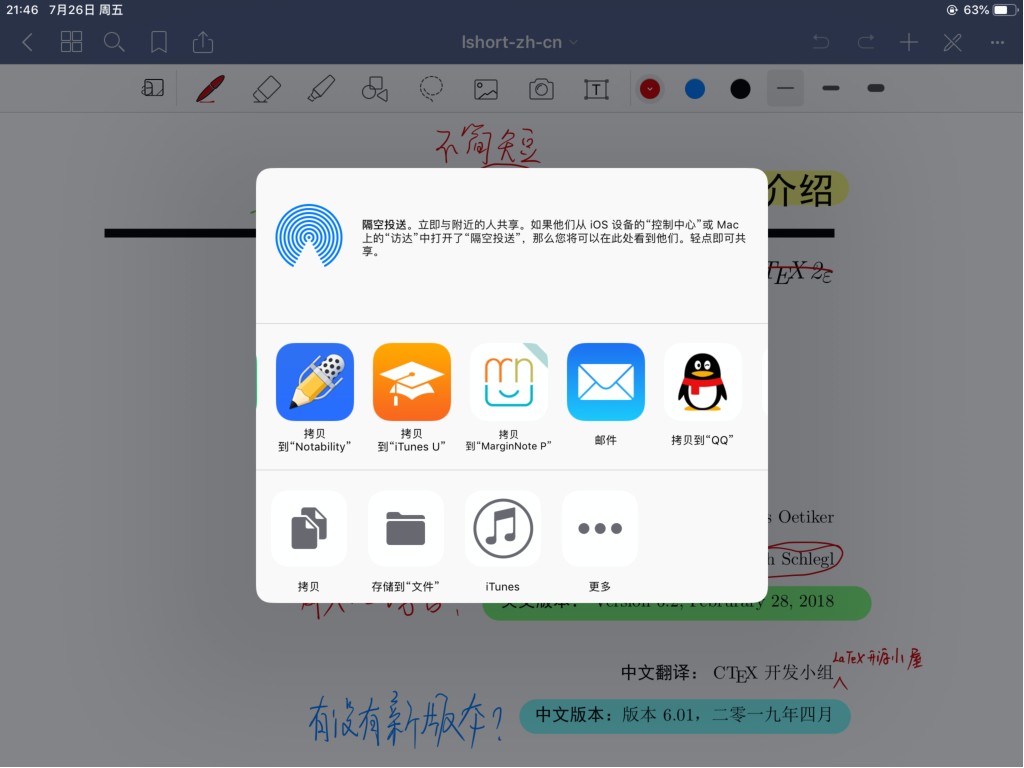
\includegraphics[width=1.0\textwidth]{05goodnotes/23exportstyles}};

      \begin{scope}[x={(img1.south east)},y={(img1.north west)}]
        % %绘制坐标辅助网络
        % \draw[very thin, draw=\finegridcolor, step=0.02] (0,0) grid (1,1);
        % \draw[thin, draw=\maingridcolor, xstep=0.1, ystep=0.1] (0,0) grid (1,1);
        % \foreach \x in {0,1,...,9} {
        %   \node [anchor=north] at (\x/10,0) {\tiny 0.\x};
        % }
        % \node [anchor=north] at (1,0) {\tiny 1};

        % \foreach \y in {0,1,...,9} {
        %   \node [anchor=east] at (0,\y/10) {\tiny 0.\y};
        % }
        % \node [anchor=east] at (0,1) {\tiny 1};
        
        % 利用fit库绘制命名矩形
        \node[fit={(0.25,0.216) (0.749, 0.78)}, inner sep=0pt, draw=red, thick] (exportfmt) {};
      \end{scope}
    \end{tikzpicture}
  \end{center}
  \end{columns}
\end{frame}

\subsection{Notability}
\begin{frame}{iOS平板}{Notability}
  \begin{columns}[c]
    \column{0.45\textwidth}
    \begin{itemize}\itemsep=3pt
    \item 基本功能
      \begin{itemize}
      \item 笔记软件
      \item 支持Apple Pencil
      \item 可以\alert{批注}PDF文档
      \end{itemize}
    \item 适用平台
      \begin{itemize}
      \item iOS平板
      \item 其它平台未知
      \end{itemize}
    \item 下载链接
      \begin{itemize}
      \item Apple Store
      \end{itemize}
    \item 授权
      \begin{itemize}
      \item \alert{68.00RMB}
      \end{itemize}
    \end{itemize}
    \column{0.45\textwidth}
    
\includegraphics[height=0.75\textheight]{06notability/01appstore}
  \end{columns}
\end{frame}

\begin{frame}{iOS平板}{Notability}
  \begin{itemize}\itemsep=3pt
  \item 文件管理
    \begin{itemize}
    \item 创建文件夹
    \item 分门别类管理
    \end{itemize}
  \end{itemize}
  \begin{center}
    \begin{tikzpicture}
      \node[anchor=south west, inner sep=0](img1) at (0,0)
      {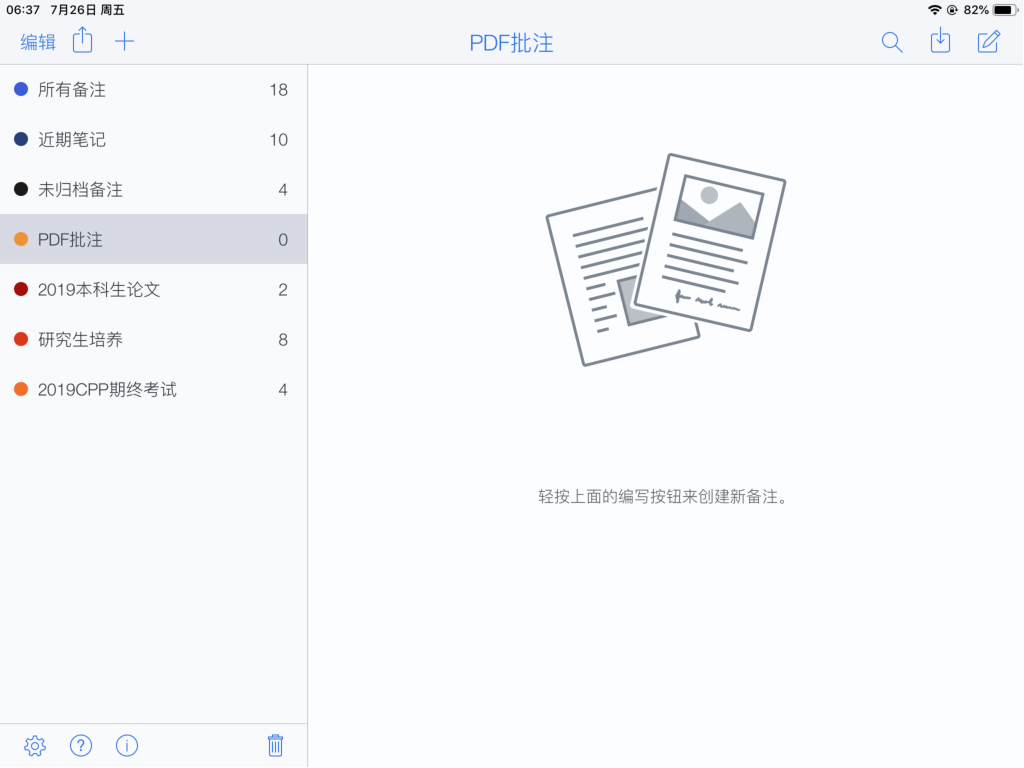
\includegraphics[width=0.5\textwidth]{06notability/02gui01}};

      \begin{scope}[x={(img1.south east)},y={(img1.north west)}]
        % % 绘制坐标辅助网络
        % \draw[very thin, draw=\finegridcolor, step=0.02] (0,0) grid (1,1);
        % \draw[thin, draw=\maingridcolor, xstep=0.1, ystep=0.1] (0,0) grid (1,1);
        % \foreach \x in {0,1,...,9} {
        %   \node [anchor=north] at (\x/10,0) {\tiny 0.\x};
        % }
        % \node [anchor=north] at (1,0) {\tiny 1};

        % \foreach \y in {0,1,...,9} {
        %   \node [anchor=east] at (0,\y/10) {\tiny 0.\y};
        % }
        % \node [anchor=east] at (0,1) {\tiny 1};
        
        % 利用fit库绘制命名矩形
        \node[fit={(0.1,0.92) (0.14, 0.97)}, inner sep=0pt, draw=blue, thick] (new) {};
        \node[fit={(0.00,0.659) (0.3, 0.72)}, inner sep=0pt, draw=red, thick] (fold) {};
        % 绘制箭头连线表示操作顺序
        \draw[-{Stealth[scale=0.8]}, blue, thick] (new.east) to [out=0,
        in=0]node[midway, sloped, above] {\tiny 创建主题}(fold.east);
      \end{scope}
    \end{tikzpicture}
  \end{center}
\end{frame}


\begin{frame}{iOS平板}{Notability}
  \begin{itemize}\itemsep=3pt
  \item 打开PDF文件
    \begin{itemize}
    \item 从邮件\enquote{附件}打开
    \end{itemize}
  \end{itemize}
  \begin{center}
    % node [midway, sloped, above] {}
    \begin{annotationimage}{width=0.5\textwidth}{06notability/02openfrommail}        
      % 利用fit库绘制命名矩形             
      \node[fit={(0.015,0.65) (0.31, 0.77)}, inner sep=0pt, draw=red, thick] (mailitem) {};
      \node[fit={(0.328,0.365) (0.5, 0.55)}, inner sep=0pt, draw=red, thick] (attachfile) {};
      \node[fit={(0.515,0.37) (0.61, 0.53)}, inner sep=0pt, draw=blue, thick] (goodnotessel) {};
      % % 绘制箭头连线表示操作顺序
      \draw[-{Stealth[scale=0.8]}, red, thick] (mailitem.south) to
      [out=-90, in=180]node [midway, sloped, below] {\small 打开邮件}
      (attachfile.west);
      
      \draw[-{Stealth[scale=0.8]}, blue, thick] (attachfile.north) to
      [out=90, in=90]node [midway, sloped, above] {\small 长按并选择
        \enquote{Notability}}  (goodnotessel.north);      
    \end{annotationimage}
  \end{center}
\end{frame}

\begin{frame}{iOS平板}{Notability}
  \begin{itemize}\itemsep=3pt
  \item 打开PDF文件
    \begin{itemize}
    \item 从\alert{Safari}\enquote{浏览器}打开
    \end{itemize}
  \end{itemize}
  \begin{center}
    % node [midway, sloped, above] {}
    \begin{annotationimage}{width=0.5\textwidth}{06notability/02openfromsafra}
    %\begin{annotationimage}[grid]{width=0.5\textwidth}{05goodnotes/06openfromsafra}          
      % 利用fit库绘制命名矩形             
      \node[fit={(0.844,0.92) (0.88, 0.97)}, inner sep=0pt, draw=red, thick] (openwithothers) {};
      \node[fit={(0.61,0.53) (0.698, 0.69)}, inner sep=0pt, draw=blue, thick] (goodnotessel) {};
      % % 绘制箭头连线表示操作顺序      
      \draw[-{Stealth[scale=0.8]}, blue, thick] (openwithothers.south) to
      [out=-90, in=90]node [midway, sloped, above] {\tiny 点按并选择}  (goodnotessel.north);      
    \end{annotationimage}
  \end{center}
\end{frame}

\begin{frame}{iOS平板}{Notability}
  \begin{itemize}\itemsep=3pt
  \item 打开PDF文件
    \begin{itemize}
    \item 从\alert{QQ}\enquote{传输文件}打开
    \end{itemize}
  \end{itemize}
  \begin{center}
    \begin{tikzpicture}
      \node[anchor=south west, inner sep=0](img1) at (0,0)
      {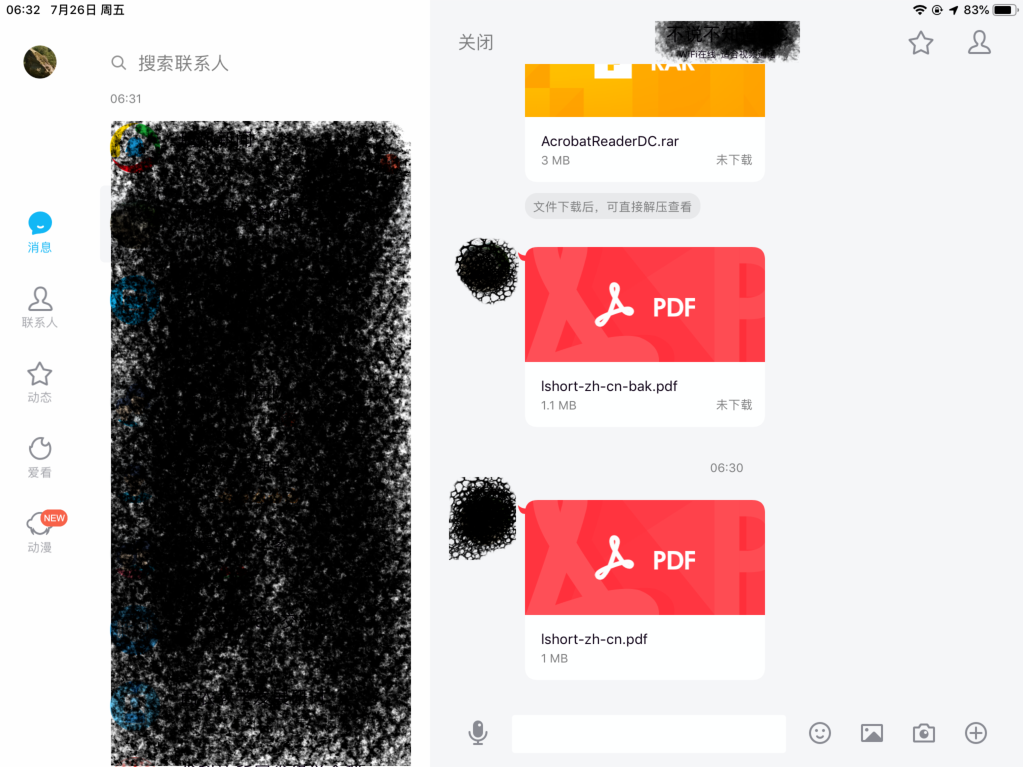
\includegraphics[width=0.34\textwidth]{06notability/03qqfile}};
      \node[anchor=south west, inner sep=0, right=0.1 of img1](img2) 
      {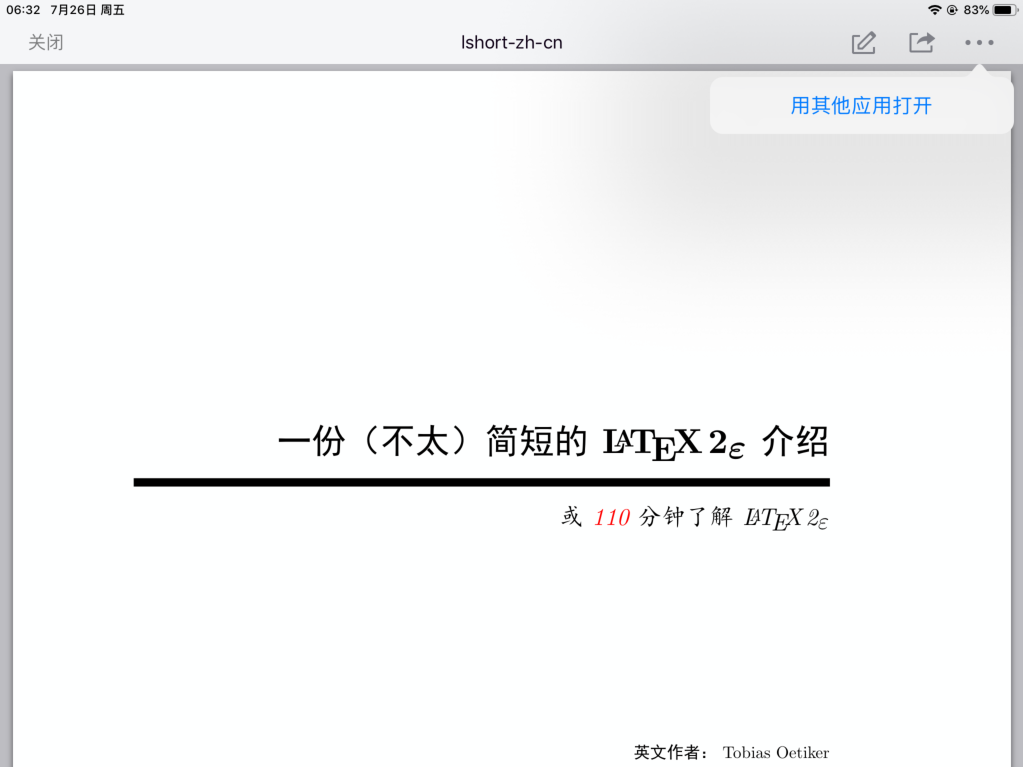
\includegraphics[width=0.34\textwidth]{06notability/03openinqq}};
      \node[anchor=south west, inner sep=0, right=0.1 of img2](img3) 
      {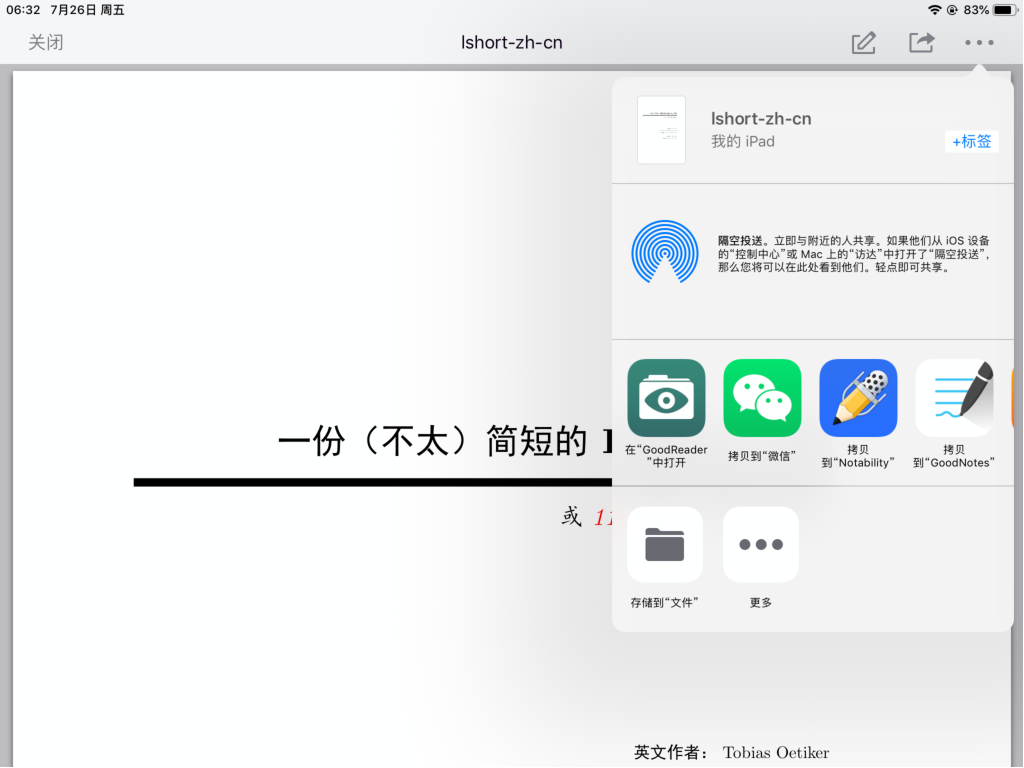
\includegraphics[width=0.34\textwidth]{06notability/03qqopenwith}};

      \begin{scope}[x={(img3.south east)},y={(img1.north west)}]
        % 绘制坐标辅助网络
        % \draw[very thin, draw=\finegridcolor, step=0.02] (0,0) grid (1,1);
        % \draw[thin, draw=\maingridcolor, xstep=0.1, ystep=0.1] (0,0) grid (1,1);
        % \foreach \x in {0,1,...,9} {
        %   \node [anchor=north] at (\x/10,0) {\tiny 0.\x};
        % }
        % \node [anchor=north] at (1,0) {\tiny 1};

        % \foreach \y in {0,1,...,9} {
        %   \node [anchor=east] at (0,\y/10) {\tiny 0.\y};
        % }
        % \node [anchor=east] at (0,1) {\tiny 1};
        
        % 利用fit库绘制命名矩形
        \node[fit={(0.14,0.11) (0.27, 0.41)}, inner sep=0pt, draw=red, thick] (qqfile) {};        
        \node[fit={(0.64,0.925) (0.66, 0.958)}, inner sep=0pt, draw=red, thick] (qqfileopen) {};
        \node[fit={(0.56,0.81) (0.662, 0.905)}, inner sep=0pt,
        draw=red, thick] (qqopenwith) {};
        \node[fit={(0.93,0.38) (0.965, 0.537)}, inner sep=0pt, draw=red, thick] (goodnotessel) {};
        
        % 绘制箭头连线表示操作顺序
        \draw[-{Stealth[scale=0.8]}, red, thick] (qqfile.east) to [out=0,
        in=180]node[midway,circle,fill=black,inner sep=0pt,minimum
        size=3pt,text=white] {\scriptsize \sffamily 1} (qqfileopen.west);
        
        \draw[-{Stealth[scale=0.8]}, red, thick] (qqfileopen.east) to
        [out=0, in=0]node[midway,circle,fill=black,inner
        sep=0pt,minimum size=3pt,text=white] {\scriptsize \sffamily 2}
        (qqopenwith.east);
        
        \draw[-{Stealth[scale=0.8]}, red, thick] (qqopenwith.east) to
        [out=0, in=180]node[midway,circle,fill=black,inner
        sep=0pt,minimum size=3pt,text=white] {\scriptsize \sffamily 3}
        (goodnotessel.west);
      \end{scope}
    \end{tikzpicture}
  \end{center}
\end{frame}

\begin{frame}{iOS平板}{Notability}
  \begin{itemize}\itemsep=3pt
  \item 打开PDF文件
    \begin{itemize}
    \item 从\alert{微信}\enquote{传输文件}打开
    \end{itemize}
  \end{itemize}
  \begin{center}
    \begin{tikzpicture}
      \node[anchor=south west, inner sep=0](img1) at (0,0)
      {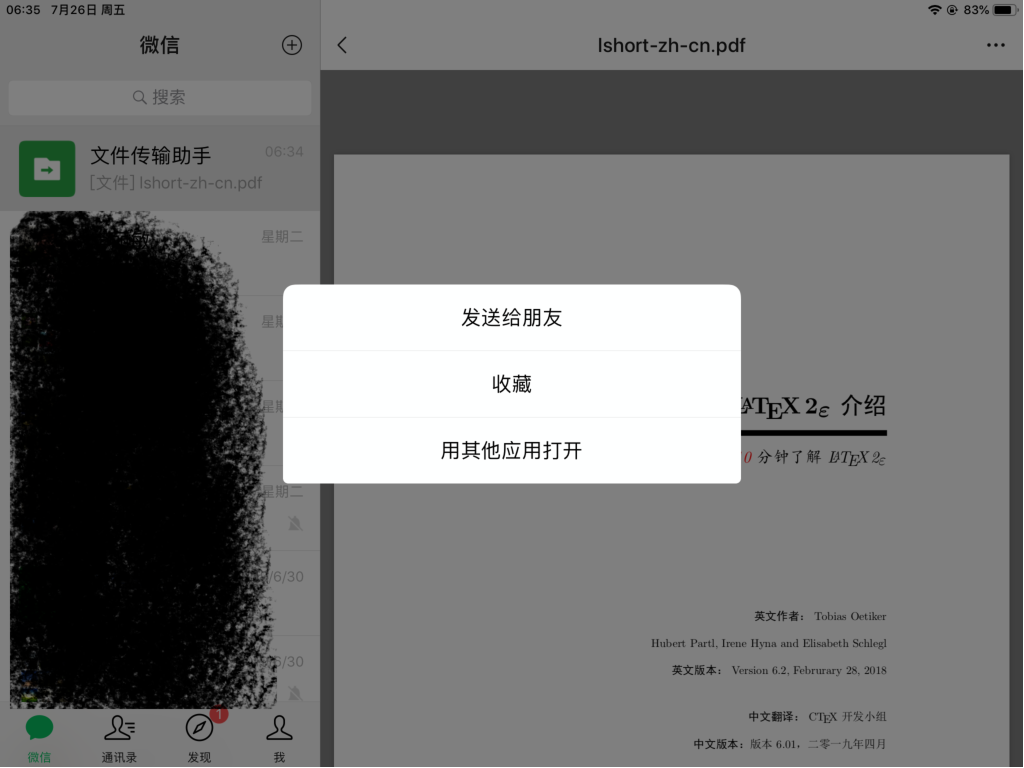
\includegraphics[width=0.48\textwidth]{06notability/04wechatopentwithmenu}};
      \node[anchor=south west, inner sep=0, right=0.1 of img1](img2) 
      {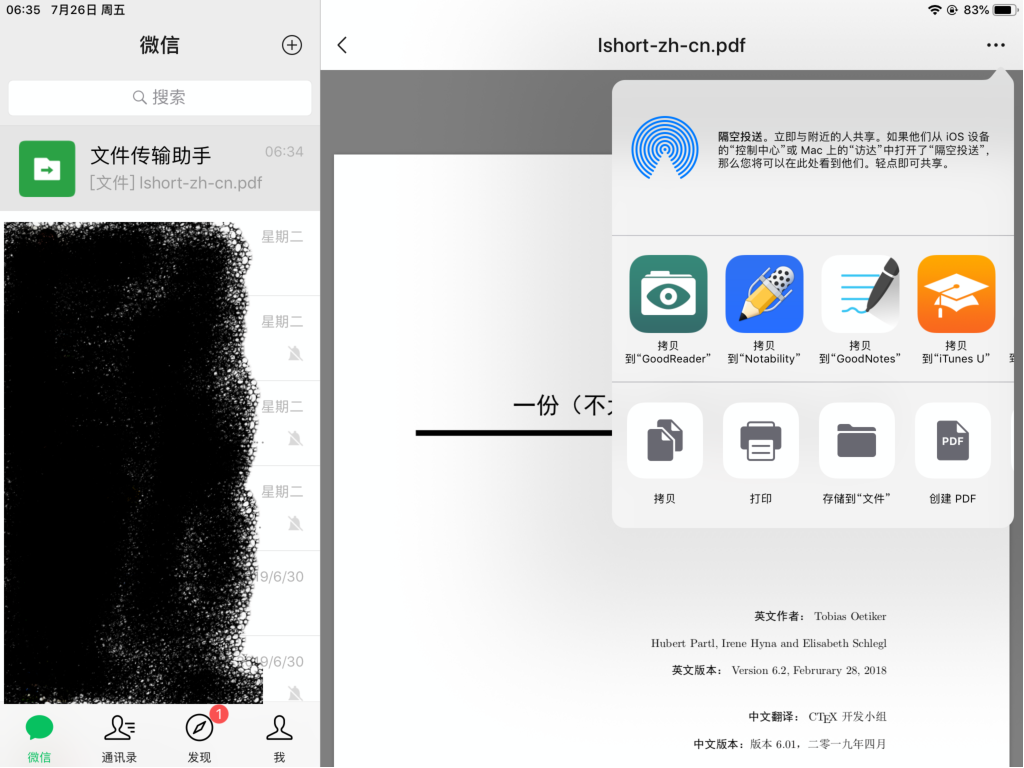
\includegraphics[width=0.48\textwidth]{06notability/04wechatopenwithgoodnotes}};

      \begin{scope}[x={(img2.south east)},y={(img1.north west)}]
        % 绘制坐标辅助网络
        % \draw[very thin, draw=\finegridcolor, step=0.02] (0,0) grid (1,1);
        % \draw[thin, draw=\maingridcolor, xstep=0.1, ystep=0.1] (0,0) grid (1,1);
        % \foreach \x in {0,1,...,9} {
        %   \node [anchor=north] at (\x/10,0) {\tiny 0.\x};
        % }
        % \node [anchor=north] at (1,0) {\tiny 1};

        % \foreach \y in {0,1,...,9} {
        %   \node [anchor=east] at (0,\y/10) {\tiny 0.\y};
        % }
        % \node [anchor=east] at (0,1) {\tiny 1};
        
        % 利用fit库绘制命名矩形
        \node[fit={(0.47,0.93) (0.495, 0.955)}, inner sep=0pt, draw=blue, thick] (others) {};        
        \node[fit={(0.135,0.364) (0.36, 0.636)}, inner sep=0pt, draw=blue, thick] (openmenu) {};
        \node[fit={(0.21,0.395) (0.285, 0.432)}, inner sep=0pt,draw=red, thick] (openwith) {};
        \node[fit={(0.852,0.52) (0.896, 0.672)}, inner sep=0pt, draw=red, thick] (goodnotessel) {};
        
        % 绘制箭头连线表示操作顺序
        \draw[-{Stealth[scale=0.8]}, blue, thick] (others.west) to [out=-135,
        in=90]node[midway,circle,fill=black,inner sep=0pt,minimum
        size=3pt,text=white] {\scriptsize \sffamily 1} (openmenu.north);
        
        \draw[-{Stealth[scale=0.8]}, red, thick] (openwith.east) to
        [out=0, in=135]node[midway,circle,fill=black,inner
        sep=0pt,minimum size=3pt,text=white] {\scriptsize \sffamily 2}
        (goodnotessel.north);
        
        % \draw[-{Stealth[scale=0.8]}, red, thick] (qqopenwith.east) to
        % [out=0, in=180]node[midway,circle,fill=black,inner
        % sep=0pt,minimum size=3pt,white] {\scriptsize \sffamily 3}
        % (goodnotessel.west);
      \end{scope}
    \end{tikzpicture}
  \end{center}
\end{frame}

\begin{frame}{iOS平板}{Notability}
  \begin{itemize}\itemsep=3pt
  \item 用Notability打开PDF文件即可将该PDF文件导入Notability
    \begin{itemize}
    \item 可选择页面(点选页面)
    \item 可选择主题(文件夹)
    \end{itemize}
  \end{itemize}
  \begin{center}
    \begin{tikzpicture}
      \node[anchor=south west, inner sep=0](img1) at (0,0)
      {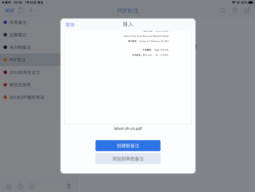
\includegraphics[width=0.34\textwidth]{06notability/05importgui01}};
      \node[anchor=south west, inner sep=0, right=0.1 of img1](img2) 
      {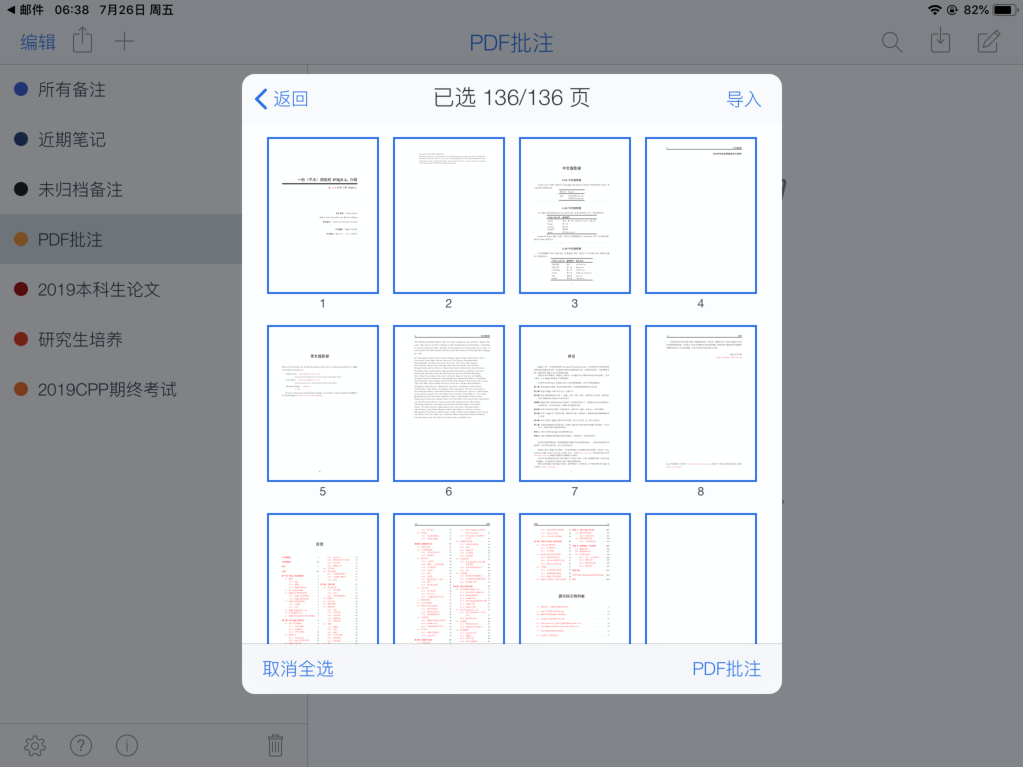
\includegraphics[width=0.34\textwidth]{06notability/05importgui02}};
      \node[anchor=south west, inner sep=0, right=0.1 of img2](img3) 
      {\includegraphics[width=0.34\textwidth]{06notability/05importgui03}};

      \begin{scope}[x={(img3.south east)},y={(img1.north west)}]
        % % 绘制坐标辅助网络
        % \draw[very thin, draw=\finegridcolor, step=0.02] (0,0) grid (1,1);
        % \draw[thin, draw=\maingridcolor, xstep=0.1, ystep=0.1] (0,0) grid (1,1);
        % \foreach \x in {0,1,...,9} {
        %   \node [anchor=north] at (\x/10,0) {\tiny 0.\x};
        % }
        % \node [anchor=north] at (1,0) {\tiny 1};

        % \foreach \y in {0,1,...,9} {
        %   \node [anchor=east] at (0,\y/10) {\tiny 0.\y};
        % }
        % \node [anchor=east] at (0,1) {\tiny 1};
        
        % 利用fit库绘制命名矩形
        \node[fit={(0.122,0.217) (0.206, 0.274)}, inner sep=0pt, draw=red, thick] (creat) {};
        \node[fit={(0.414,0.1) (0.586, 0.9)}, inner sep=0pt, draw=red, thick] (open) {};
        \node[fit={(0.556,0.115) (0.581, 0.148)}, inner sep=0pt, draw=blue, thick] (sel) {};
        \node[fit={(0.750,0.731) (0.922, 0.772)}, inner sep=0pt, draw=red, thick] (fold) {};

        % \node[fit={(0.565,0.85) (0.582, 0.89)}, inner sep=0pt,
        % draw=blue, fill = green!30, thick, opacity = 0.3] (import) {};
        
        % 绘制箭头连线表示操作顺序
        \draw[-{Stealth[scale=0.8]}, blue, thick] (creat.east) to [out=0,
        in=180] (open.west);

        \draw[-{Stealth[scale=0.8]}, red, thick] (sel.east) to [out=0,
        in=180] (fold.west);
      \end{scope}
    \end{tikzpicture}
  \end{center}
\end{frame}

\begin{frame}{iOS平板}{Notability}
  \begin{itemize}\itemsep=3pt
  \item 批注PDF文件
    \begin{itemize}
    \item 在批注工具栏中\alert{选择合适工具}进行批注
    \end{itemize}
  \end{itemize}
  \begin{center}
    \begin{annotationimage}{width=0.5\textwidth}{06notability/02gui02}
    %\begin{annotationimage}[grid]{width=0.5\textwidth}{05goodnotes/10toolbar}          
      % 利用fit库绘制命名矩形             
      \node[fit={(0.01,0.91) (0.99, 0.97)}, inner sep=0pt, draw=red, thick] (pdffold) {};
      \draw[annotation right = {批注工具栏 at 0.94}] to (0.97,0.94);
    \end{annotationimage}
  \end{center}
\end{frame}

\begin{frame}{iOS平板}{Notability}
  \begin{itemize}\itemsep=3pt
  \item 批注PDF文件
    \begin{itemize}
    \item 利用\alert{放大镜}工具实现细节批注
    \end{itemize}
  \end{itemize}
  \begin{center}
    \begin{tikzpicture}
      \node[anchor=south west, inner sep=0](img1) at (0,0)
      {\includegraphics[width=0.48\textwidth]{06notability/02gui02}};
      \node[anchor=south west, inner sep=0, right=0.1 of img1](img2) 
      {\includegraphics[width=0.48\textwidth]{06notability/11magnifier}};

      \begin{scope}[x={(img2.south east)},y={(img1.north west)}]
        % 绘制坐标辅助网络
        % \draw[very thin, draw=\finegridcolor, step=0.02] (0,0) grid (1,1);
        % \draw[thin, draw=\maingridcolor, xstep=0.1, ystep=0.1] (0,0) grid (1,1);
        % \foreach \x in {0,1,...,9} {
        %   \node [anchor=north] at (\x/10,0) {\tiny 0.\x};
        % }
        % \node [anchor=north] at (1,0) {\tiny 1};

        % \foreach \y in {0,1,...,9} {
        %   \node [anchor=east] at (0,\y/10) {\tiny 0.\y};
        % }
        % \node [anchor=east] at (0,1) {\tiny 1};
        
        % 利用fit库绘制命名矩形
        \node[fit={(0.472,0.00) (0.498, 0.062)}, inner sep=0pt, draw=blue, thick] (icon) {};
        \node[fit={(0.853,0.570) (0.988, 0.666)}, inner sep=0pt, draw=red, thick] (roi) {};
        \node[fit={(0.504,0.00) (1.00, 0.397)}, inner sep=0pt, draw=blue, thick] (magnifier) {};        
        
        % 绘制箭头连线表示操作顺序
        \draw[-{Stealth[scale=0.8]}, red, thick] (icon.north) to [out=90,
        in=180]node[midway,circle,fill=black,inner sep=0pt,minimum
        size=3pt,text=white] {\scriptsize \sffamily 1} (roi.west);

        \draw[-{Stealth[scale=0.8]}, blue, thick] (roi.east) to [out=0,
        in=0]node[midway,circle,fill=black,inner sep=0pt,minimum
        size=3pt,text=white] {\scriptsize \sffamily 2} (magnifier.east);
      \end{scope}
    \end{tikzpicture}
  \end{center}
\end{frame}

\begin{frame}{iOS平板}{Notability}
  \begin{itemize}\itemsep=3pt
  \item \enquote{批注}工具栏
    \begin{itemize}
    \item 工具类型
    \item 工具属性
    \end{itemize}
  \end{itemize}
  \begin{center}
    \begin{annotationimage}{width=0.8\textwidth}{06notability/02toolbar}
    %\begin{annotationimage}[grid]{width=0.8\textwidth}{06notability/02toolbar}      
      % 添加各图标标注
      \foreach \ann/\xpos in
      {
        {导\\出\\工\\具}/0.07, {撤\\消\\工\\具}/0.24,
        {文\\字\\工\\具}/0.402, {铅\\笔\\工\\具}/0.44,
        {萤\\光\\笔\\工\\具}/0.48, {橡\\皮\\擦\\工\\具}/0.52, 
        {索\\套\\选\\择\\工\\具}/0.56, {移\\动\\工\\具}/0.595,
        {录\\音\\工\\具}/0.735, {插\\入\\素\\材\\工\\具}/0.9,
        {属\\性\\设\\置}/0.94, {页\\面\\边\\栏}/0.975
      }
      {
        \draw[annotation below = {{\ann} at \xpos}] to (\xpos,0.30);
      }
    \end{annotationimage}
  \end{center}
\end{frame}

\begin{frame}{iOS平板}{Notability}
  \begin{itemize}\itemsep=3pt
  \item \enquote{批注}工具属性设置
    \begin{itemize}
    \item 点按工具图标\alert{两次}进行工具设置
    \item 在属性设计区设置颜色、宽度等属性
    \end{itemize}
  \end{itemize}
  \vspace{-1.5ex}
  \begin{center}
    \begin{tikzpicture}[font=\small]
      \node[anchor=south west, inner sep=0](img1) at (0,0)
      {\includegraphics[width=0.45\textwidth]{06notability/10textcol}};
      
      \node[anchor=south west, inner sep=0, right=0.1 of img1](img2) 
      {\includegraphics[width=0.45\textwidth]{06notability/10textfmt}};

      \node[anchor=west, inner sep=2pt, above=0.2 of img2,xshift = -3.25cm,draw,blue,thick](txt)
      {文字属性设置};

      \begin{scope}[x={(img2.south east)},y={(img1.north west)}]
        % %绘制坐标辅助网络
        % \draw[very thin, draw=\finegridcolor, step=0.02] (0,0) grid (1,1);
        % \draw[thin, draw=\maingridcolor, xstep=0.1, ystep=0.1] (0,0) grid (1,1);
        % \foreach \x in {0,1,...,9} {
        %   \node [anchor=north] at (\x/10,0) {\tiny 0.\x};
        % }
        % \node [anchor=north] at (1,0) {\tiny 1};

        % \foreach \y in {0,1,...,9} {
        %   \node [anchor=east] at (0,\y/10) {\tiny 0.\y};
        % }
        % \node [anchor=east] at (0,1) {\tiny 1};
        
        % 利用fit库绘制命名矩形
        \node[fit={(0.195,0.60) (0.302, 0.90)}, inner sep=0pt, draw=red, thick] (txtcol) {}; 
        \node[fit={(0.515,0.52) (0.924, 0.573)}, inner sep=0pt, draw=red, thick] (txtfmt) {};
        % % 绘制箭头连线表示操作顺序
        \draw[-{Stealth[scale=0.8]}, red, thick] (txt.west) to [out=180,
        in=90]node[midway, sloped, above] {文字颜色} (txtcol.north);

        \draw[-{Stealth[scale=0.8]}, red, thick] (txt.east) to [out=0,
        in=90]node[midway, sloped, above] {文字样式} (txtfmt.north);
      \end{scope}
    \end{tikzpicture}
  \end{center}
\end{frame}

\begin{frame}{iOS平板}{Notability}
  \begin{itemize}\itemsep=3pt
  \item \enquote{批注}工具属性设置
    \begin{itemize}
    \item 点按工具图标\alert{两次}进行工具设置
    \item 在属性设计区设置颜色、宽度等属性
    \end{itemize}
  \end{itemize}
  \vspace{-1ex}
  \begin{center}
    \begin{tikzpicture}[font=\small]
      \node[anchor=south west, inner sep=0](img1) at (0,0)
      {\includegraphics[width=0.48\textwidth]{06notability/06pen}};

      \node[anchor=south west, inner sep=2pt, above=0.2 of img1,draw,blue,thick](txt)
      {铅笔属性};
    \end{tikzpicture}
  \end{center}
\end{frame}

\begin{frame}{iOS平板}{Notability}
  \begin{itemize}\itemsep=3pt
  \item \enquote{批注}工具属性设置
    \begin{itemize}
    \item 点按工具图标\alert{两次}进行工具设置
    \item 在属性设计区设置颜色、宽度等属性
    \end{itemize}
  \end{itemize}
  \vspace{-1ex}
  \begin{center}
    \begin{tikzpicture}[font=\small]
      \node[anchor=south west, inner sep=0](img1) at (0,0)
      {\includegraphics[width=0.48\textwidth]{06notability/07highlightpen}};

      \node[anchor=south west, inner sep=2pt, above=0.2 of img1,draw,blue,thick](txt)
      {萤光笔属性};
    \end{tikzpicture}
  \end{center}
\end{frame}

\begin{frame}{iOS平板}{Notability}
  \begin{itemize}\itemsep=3pt
  \item \enquote{批注}工具属性设置
    \begin{itemize}
    \item 点按工具图标\alert{两次}进行工具设置
    \item 在属性设计区设置颜色、宽度等属性
    \end{itemize}
  \end{itemize}
  \vspace{-1ex}
  \begin{center}
    \begin{tikzpicture}[font=\small]
      \node[anchor=south west, inner sep=0](img1) at (0,0)
      {\includegraphics[width=0.48\textwidth]{06notability/08eraser}};

      \node[anchor=south west, inner sep=2pt, above=0.2 of img1,draw,blue,thick](txt)
      {橡皮擦属性};
    \end{tikzpicture}
  \end{center}
\end{frame}

\begin{frame}{iOS平板}{Notability}
  \begin{itemize}\itemsep=3pt
  \item \enquote{批注}工具属性设置
    \begin{itemize}
    \item 点按工具图标\alert{两次}进行工具设置
    \item 在属性设计区设置颜色、宽度等属性
    \end{itemize}
  \end{itemize}
  \vspace{-1ex}
  \begin{center}
    \begin{tikzpicture}[font=\small]
      \node[anchor=south west, inner sep=0](img1) at (0,0)
      {\includegraphics[width=0.48\textwidth]{06notability/09seltool}};

      \node[anchor=south west, inner sep=2pt, above=0.2 of img1,draw,blue,thick](txt)
      {索套属性};
    \end{tikzpicture}
  \end{center}
\end{frame}

\begin{frame}{iOS平板}{Notability}
  \begin{columns}[T]
    \column{0.4\textwidth}
  \begin{itemize}\itemsep=8pt
  \item \enquote{\alert{导出}}批注结果
    \begin{itemize}\itemsep=8pt
    \item 选择发送方式
      \begin{itemize}\itemsep=10pt
      \item 邮件(\alert{强烈推荐})
      \item 网盘(\alert{不}推荐)
      \item iTunes  
      \item 其它应用\\
        --微信\\--QQ\\--\ldots
      \item \ldots
      \end{itemize}
    \end{itemize}
  \end{itemize}
    \column{0.55\textwidth}
  \begin{center}
    \begin{tikzpicture}[font=\small]
      \node[anchor=south west, inner sep=0](img1) at (0,0)
      {\includegraphics[width=1.00\textwidth]{06notability/12exportmenu}};

      \begin{scope}[x={(img1.south east)},y={(img1.north west)}]
        % %绘制坐标辅助网络
        % \draw[very thin, draw=\finegridcolor, step=0.02] (0,0) grid (1,1);
        % \draw[thin, draw=\maingridcolor, xstep=0.1, ystep=0.1] (0,0) grid (1,1);
        % \foreach \x in {0,1,...,9} {
        %   \node [anchor=north] at (\x/10,0) {\tiny 0.\x};
        % }
        % \node [anchor=north] at (1,0) {\tiny 1};

        % \foreach \y in {0,1,...,9} {
        %   \node [anchor=east] at (0,\y/10) {\tiny 0.\y};
        % }
        % \node [anchor=east] at (0,1) {\tiny 1};
        
        % 利用fit库绘制命名矩形
        \node[fit={(0.05,0.92) (0.088, 0.97)}, inner sep=0pt, draw=blue, thick] (export) {}; 
        \node[fit={(0.01,0.202) (0.393, 0.9)}, inner sep=0pt, draw=red, thick] (menu) {};
        % % 绘制箭头连线表示操作顺序
        \draw[-{Stealth[scale=0.8]}, blue, thick] (export.east) to [out=0,
        in=90] (menu.north);
      \end{scope}
    \end{tikzpicture}
  \end{center}
  \end{columns}
\end{frame}

\begin{frame}{iOS平板}{Notability}
  \begin{columns}[T]
    \column{0.4\textwidth}
  \begin{itemize}\itemsep=3pt
  \item \enquote{\alert{导出}}批注结果
    \begin{itemize}\itemsep=3pt
    \item 电子邮件导出
      \begin{itemize}\itemsep=8pt
      \item 格式---PDF
      \item PDF选项
      \item \ldots
      \end{itemize}
    \end{itemize}
  \end{itemize}
  %\vspace{-1.5ex}
  \column{0.55\textwidth}
  \begin{center}
    \begin{tikzpicture}[font=\small]
      \node[anchor=south west, inner sep=0](img1) at (0,0)
      {\includegraphics[width=1.00\textwidth]{06notability/13exportemail}};

      \begin{scope}[x={(img1.south east)},y={(img1.north west)}]
        % %绘制坐标辅助网络
        % \draw[very thin, draw=\finegridcolor, step=0.02] (0,0) grid (1,1);
        % \draw[thin, draw=\maingridcolor, xstep=0.1, ystep=0.1] (0,0) grid (1,1);
        % \foreach \x in {0,1,...,9} {
        %   \node [anchor=north] at (\x/10,0) {\tiny 0.\x};
        % }
        % \node [anchor=north] at (1,0) {\tiny 1};

        % \foreach \y in {0,1,...,9} {
        %   \node [anchor=east] at (0,\y/10) {\tiny 0.\y};
        % }
        % \node [anchor=east] at (0,1) {\tiny 1};
        
        % 利用fit库绘制命名矩形
        \node[fit={(0.05,0.92) (0.088, 0.97)}, inner sep=0pt, draw=blue, thick] (export) {}; 
        \node[fit={(0.01,0.202) (0.393, 0.9)}, inner sep=0pt, draw=red, thick] (menu) {};
        % % 绘制箭头连线表示操作顺序
        \draw[-{Stealth[scale=0.8]}, blue, thick] (export.east) to [out=0,
        in=90] (menu.north);
      \end{scope}
    \end{tikzpicture}
  \end{center}
  \end{columns}
\end{frame}

\begin{frame}{iOS平板}{Notability}
  \begin{columns}[T]
    \column{0.4\textwidth}
  \begin{itemize}\itemsep=3pt
  \item \enquote{\alert{导出}}批注结果
    \begin{itemize}\itemsep=3pt
    \item 其它应用导出
      \begin{itemize}\itemsep=8pt
      \item 微信
      \item QQ
      \item GoodReader
      \item \ldots
      \end{itemize}
    \end{itemize}
  \end{itemize}
  %\vspace{-1.5ex}
  \column{0.55\textwidth}
  \begin{center}
    \begin{tikzpicture}[font=\small]
      \node[anchor=south west, inner sep=0](img1) at (0,0)
      {\includegraphics[width=1.00\textwidth]{06notability/14exportothersel}};

      \begin{scope}[x={(img1.south east)},y={(img1.north west)}]
        % %绘制坐标辅助网络
        % \draw[very thin, draw=\finegridcolor, step=0.02] (0,0) grid (1,1);
        % \draw[thin, draw=\maingridcolor, xstep=0.1, ystep=0.1] (0,0) grid (1,1);
        % \foreach \x in {0,1,...,9} {
        %   \node [anchor=north] at (\x/10,0) {\tiny 0.\x};
        % }
        % \node [anchor=north] at (1,0) {\tiny 1};

        % \foreach \y in {0,1,...,9} {
        %   \node [anchor=east] at (0,\y/10) {\tiny 0.\y};
        % }
        % \node [anchor=east] at (0,1) {\tiny 1};
        
        % 利用fit库绘制命名矩形
        \node[fit={(0.05,0.92) (0.088, 0.97)}, inner sep=0pt, draw=blue, thick] (export) {}; 
        \node[fit={(0.01,0.312) (0.402, 0.9)}, inner sep=0pt, draw=red, thick] (menu) {};
        % % 绘制箭头连线表示操作顺序
        \draw[-{Stealth[scale=0.8]}, blue, thick] (export.east) to [out=0,
        in=90] (menu.north);
      \end{scope}
    \end{tikzpicture}
  \end{center}
  \end{columns}
\end{frame}

\begin{frame}[standout,plain]
  说明:\\  
  只要\alert{熟悉一个}就好\\
  手写能够留下\alert{真迹}\\
  肯定还有你偏好的其它软件
\end{frame}

\section{\LaTeX 源码修订}
\subsection{changes宏包}

\begin{frame}{\LaTeX 源码修订}{changes宏包}
    \begin{columns}[T]
    \column{0.35\textwidth}
    \begin{itemize}\itemsep=8pt
    \item 基本功能
      \begin{itemize}
      \item \LaTeX 源码级批注
      \end{itemize}
    \item 适用平台
      \begin{itemize}
      \item \LaTeX 运行平台
      \end{itemize}
    \item 下载链接
      \begin{itemize}
      \item \LaTeX 发行版自带
      \end{itemize}
    \item 授权
      \begin{itemize}
      \item \alert{免费}
      \end{itemize}
    \end{itemize}
    \column{0.55\textwidth}
    \centering
    \includegraphics[height=0.8\textheight]{07changes/01changes}
  \end{columns}
\end{frame}

\begin{frame}{\LaTeX 源码修订}{changes宏包}
  \begin{columns}[T]
    \column{0.45\textwidth}
    \begin{itemize}\itemsep=8pt
    \item 修订步骤
      \begin{itemize}\itemsep=10pt
      \item 引入changes宏包
      \item 设置审阅人属性
      \item 标记修订内容
      \item 高亮显示和添加批注
      \item 用\LaTeX 对源文档进行排版
      \item 输出修订列表
      \item 接受/拒绝修订后删除各类标记
      \end{itemize}
    \end{itemize}
    \column{0.45\textwidth} \centering
    \includegraphics[height=0.6\textheight]{07changes/02changesscheme}        
  \end{columns}
\end{frame}

\begin{frame}{\LaTeX 源码修订}{changes宏包}
  \begin{itemize}%\itemsep=8pt
  \item 修订命令\footnote[frame,1]{详情请用:\enquote{\alert{texdoc changes}命令}查阅宏
      包说明书。}
    \begin{itemize}%\itemsep=10pt
    \item 审阅人设置命令
      \begin{itemize}
      \item \texinline{\definechangesauthor[name=<name>, color=<color>]{<id>}}
      \end{itemize}
    \item 修订命令
      \begin{itemize}
      \item \texinline{\added[id=<id>, comment=<comment>]{<new text>}}
      \item \texinline{\deleted[id=<id>, comment=<comment>]{<old text>}}
      \item \texinline{\replaced[id=<id>, comment=<comment>]{<new text>}{<old text>}}  
      \item \texinline{\highlight[id=<id>, comment=<comment>]{<text>}}
      \item \texinline{\comment[id=<id>]{<comment>}}  
      \end{itemize}
    \item 输出修订列表命令
      \begin{itemize}
      \item \texinline{\listofchanges[style=<style>, title=<title>, show=<type>]}
      \end{itemize}
    \item 宏包选项
    \item 标记设置命令
    \item 其它命令
    \end{itemize}
  \end{itemize}
\end{frame}

\begin{frame}[standout,plain]
  类似的宏包还有:\\
  easyReview\\
  todonotes\\
  pdfreview\\...\\
  请用\enquote{\alert{texdoc}}命令查看其说明书
\end{frame}

%\section{小结}
\begin{frame}[standout,plain]
  PDF批注方案很多\\
  根据习惯选用即可\\
  这个文档\\
  肯定有不完善的地方\\
  欢迎批评指正\\...
\end{frame}

\end{document}

% \begin{frame}{\LaTeX 源码修订}{changes宏包}
  
% \end{frame}

%[label=testframe]

%%% Local Variables:
%%% mode: latex
%%% TeX-master: t
%%% End:
